% ============================================================
% Chapitre 6 : Réalisation, Tests et Déploiement
% ============================================================

\section{Introduction}

À l'issue des phases d'analyse des besoins et de conception architecturale, ce chapitre décrit
la concrétisation technique de la plateforme \textbf{RevMine}. Il couvre l'ensemble du processus
de réalisation~: de la mise en place de la culture DevOps et de l'environnement de développement
jusqu'à l'implémentation des différents modules du système, en passant par la stratégie de test,
le déploiement et la surveillance de la plateforme.

L'objectif de cette phase est de produire une application capable de centraliser la configuration
des espaces de travail, de collecter les données issues des plateformes de gestion de code, de les
nettoyer et de les structurer, puis de générer des analyses visuelles exploitables. Pour répondre
à ces exigences, une architecture microservices a été adoptée, avec une séparation claire des
responsabilités entre l'API Gateway, les services métier, les mécanismes de communication
asynchrone et les composants d'infrastructure.

Ce chapitre s'organise selon le plan suivant~:

\begin{enumerate}
    \item \textbf{Environnement de développement}~: présentation du matériel et des outils utilisés~;
    \item \textbf{Technologies utilisées}~: justification des choix techniques retenus~;
    \item \textbf{Culture DevOps}~: principes et pratiques adoptés tout au long du cycle de vie~;
    \item \textbf{Planification}~: méthodologie Scrum et gestion des tâches via le tableau Kanban~;
    \item \textbf{Développement}~: implémentation des microservices backend, du frontend, de la
          communication inter-services et des mesures de sécurité~;
    \item \textbf{Build}~: conteneurisation de chaque service via Docker~;
    \item \textbf{Test}~: stratégie de validation multi-niveaux (unitaire, intégration, end-to-end,
          qualité statique)~;
    \item \textbf{Déploiement}~: orchestration avec Docker Compose et pipeline CI/CD GitLab~;
    \item \textbf{Surveillance}~: observabilité via la pile Grafana~+~Loki~+~Promtail.
\end{enumerate}

% ============================================================
\section{Environnement de développement}
% ============================================================

\subsection{Matériel}

Le développement de RevMine a été mené en binôme sur deux postes de travail locaux. Le
Tableau~\ref{tab:env-dev} récapitule leurs configurations matérielles et logicielles.

\begin{table}[H]
\centering
\small
\caption{Configurations des postes de développement}
\label{tab:env-dev}
\begin{tabular}{|>{\raggedright\arraybackslash}p{3.5cm}
                |>{\raggedright\arraybackslash}p{5cm}
                |>{\raggedright\arraybackslash}p{5cm}|}
\hline
\textbf{Caractéristique} & \textbf{Poste 1} & \textbf{Poste 2} \\
\hline
Système d'exploitation & Windows 11 Pro (64~bits) & Windows 11 Pro (64~bits) \\
\hline
Processeur & Intel Core i5 -- 10\textsuperscript{e} génération
           & Intel Core i7 -- 10\textsuperscript{e} génération \\
\hline
Carte graphique & NVIDIA GeForce GTX~1650 & -- \\
\hline
Mémoire RAM & 8~Go & 16~Go \\
\hline
Stockage & SSD 256~Go & SSD 512~Go \\
\hline
\end{tabular}
\end{table}

\subsection{Logiciels et outils}

Les principaux outils utilisés au cours du développement sont les suivants~:

\begin{itemize}
    \item \textbf{Visual Studio Code} et \textbf{PyCharm Community Edition}~: éditeurs utilisés
          respectivement pour le développement frontend/backend généraliste et pour le développement
          Python spécialisé~;
    \item \textbf{Docker Desktop}~: plateforme de conteneurisation permettant d'exécuter et
          d'orchestrer l'ensemble des services sous Windows~;
    \item \textbf{Postman}~: outil de test et de documentation des API REST~;
    \item \textbf{Git / GitLab}~: système de gestion de versions distribué, utilisé pour le
          versioning, la gestion des branches et le suivi du projet~;
    \item \textbf{pgAdmin 4}~: interface graphique d'administration des bases de données
          PostgreSQL.
\end{itemize}

% ============================================================
\section{Technologies utilisées}
% ============================================================

\subsection{Python}
\begin{wrapfigure}{r}{0.1\textwidth}
    \centering
    
\includegraphics[width=0.1\textwidth]{assets/python_logo.png}
\end{wrapfigure}

Python est un langage de programmation interprété, multiparadigme et open source, reconnu pour
sa lisibilité, sa flexibilité et la richesse de son écosystème \parencite{pythonWhatPython}. Sa
syntaxe épurée réduit le coût de maintenance des projets, tandis que ses bibliothèques spécialisées
couvrent de nombreux domaines, de l'analyse de données à l'apprentissage automatique. Dans
RevMine, Python constitue le socle du développement backend en raison de sa maturité pour
l'interaction avec les API REST, le traitement de données et l'intégration de services
d'intelligence artificielle.

\subsection{Django et Django REST Framework}
\begin{wrapfigure}{r}{0.1\textwidth}
    \centering
    
\includegraphics[width=0.1\textwidth]{assets/django_logo.png}
\end{wrapfigure}

Django est un framework web Python suivant le paradigme Modèle-Vue-Template (MVT). Il intègre
nativement un ORM\footnote{ORM (\textit{Object-Relational Mapping})~: technique de correspondance
entre les objets d'un programme et les tables d'une base de données relationnelle, permettant de
manipuler les données sans écrire de requêtes SQL.} puissant, un système d'authentification
robuste et une interface d'administration \parencite{holovaty2009django}. Son extension Django
REST Framework (DRF) facilite la conception d'API RESTful performantes et bien documentées. Ce
framework a été retenu pour les services nécessitant une gestion complexe des données métier --
notamment l'API Gateway, le service de configuration, le service de collecte et le service
d'analyse -- en raison de son architecture modulaire, de son ORM adapté à PostgreSQL et de ses
mécanismes de sécurité intégrés.

\subsection{FastAPI}
\begin{wrapfigure}{r}{0.1\textwidth}
    \centering
    
\includegraphics[width=0.1\textwidth]{assets/fastapi_logo.png}
\end{wrapfigure}

FastAPI est un framework Python moderne orienté performances, reposant sur les annotations de
type Python~3.7+ et le paradigme asynchrone (\texttt{async/await}) \parencite{ramirez2021fastapi}.
Il génère automatiquement une documentation interactive (Swagger UI, ReDoc) et assure la
validation des données via Pydantic. Sa légèreté et sa réactivité native en font un choix adapté
au service LLM de RevMine, pour lequel la rapidité de réponse et la simplicité de l'interface
sont prioritaires.

\subsection{Go et WebSocket}
\begin{wrapfigure}{r}{0.1\textwidth}
    \centering
    
\includegraphics[width=0.1\textwidth]{assets/go_logo.png}
\end{wrapfigure}

Go est un langage compilé et statiquement typé, développé par Google, dont la gestion native de
la concurrence via les \textit{goroutines} en fait un choix de référence pour les services à haute
concurrence et faible latence \parencite{go2012donovan}. Le service de notification de RevMine
doit gérer simultanément un grand nombre de connexions persistantes en temps réel~; Go répond à
cette contrainte en permettant le traitement de milliers de connexions concurrentes avec une
empreinte mémoire réduite. Le framework \textbf{Fiber}, inspiré d'Express.js, a été utilisé pour
simplifier le développement des API REST associées.

Le protocole \textbf{WebSocket}\footnote{WebSocket (RFC~6455)~: protocole de communication
standardisé établissant un canal bidirectionnel et persistant entre un client et un serveur sur
une connexion TCP, contrairement à HTTP qui est unidirectionnel par nature.} établit un canal de
communication bidirectionnel et persistant, permettant au service de notification de diffuser
instantanément les événements système (démarrage de collecte, fin d'analyse, erreur) aux clients
connectés, sans recourir au \textit{polling} HTTP.

\subsection{React.js}
\begin{wrapfigure}{r}{0.1\textwidth}
    \centering
    
\includegraphics[width=0.1\textwidth]{assets/react_logo.png}
\end{wrapfigure}

React.js est une bibliothèque JavaScript open source développée par Meta pour la construction
d'interfaces utilisateur interactives, reposant sur une architecture en composants réutilisables
et une gestion efficace du DOM virtuel \parencite{facebookReact2023}. Dans RevMine, React.js
assure le développement de l'interface utilisateur, permettant l'exploration interactive des
données, la configuration des collectes et la visualisation des résultats d'analyse.

\subsection{Tailwind CSS}
\begin{wrapfigure}{r}{0.1\textwidth}
    \centering
    
\includegraphics[width=0.1\textwidth]{assets/tailwind_logo.png}
\end{wrapfigure}

Tailwind CSS est un framework CSS \textit{utility-first} qui permet de construire des interfaces
modernes et responsives directement dans le balisage, sans rédiger de feuilles de style
personnalisées volumineuses \parencite{tailwindlabs2023}. Son approche par classes utilitaires
composables favorise la cohérence visuelle et s'intègre naturellement avec React.

\subsection{Docker}
\begin{wrapfigure}{r}{0.1\textwidth}
    \centering
    
\includegraphics[width=0.1\textwidth]{assets/docker_logo.png}
\end{wrapfigure}

Docker est une plateforme de conteneurisation permettant d'empaqueter une application et ses
dépendances dans un conteneur léger, portable et isolé \parencite{merkel2014docker}. Un
\textit{conteneur} est une unité d'exécution autonome qui encapsule le code, les bibliothèques
et les configurations nécessaires au fonctionnement d'un service, garantissant ainsi un
comportement identique quel que soit l'environnement d'exécution. Docker Compose étend cette
capacité en orchestrant plusieurs services applicatifs et d'infrastructure de manière
déclarative. Dans RevMine, Docker assure la conteneurisation de l'ensemble des services,
garantissant la reproductibilité des environnements entre le développement, les tests et le
déploiement.

\subsection{PostgreSQL}
\begin{wrapfigure}{r}{0.1\textwidth}
    \centering
    
\includegraphics[width=0.1\textwidth]{assets/postgresql_logo.png}
\end{wrapfigure}

PostgreSQL est un système de gestion de base de données relationnelle objet open source, reconnu
pour sa robustesse, sa conformité aux standards SQL et ses fonctionnalités avancées
\parencite{postgresql2023}. Son intégration native avec l'ORM Django facilite la persistance des
données métier. Chaque microservice de RevMine dispose de sa propre base PostgreSQL, assurant
ainsi l'isolation des données et limitant les dépendances directes entre services.

\subsection{MinIO}
\begin{wrapfigure}{r}{0.1\textwidth}
    \centering
    
\includegraphics[width=0.1\textwidth]{assets/minio_logo.png}
\end{wrapfigure}

MinIO est une solution de stockage objet haute performance compatible avec l'API Amazon S3,
conçue pour le stockage de fichiers volumineux et de données semi-structurées
\parencite{minio2023}. Dans RevMine, MinIO archive les données brutes collectées depuis GitHub et
GitLab sous forme de fichiers JSON, séparant ainsi les artefacts bruts du stockage relationnel et
facilitant leur réutilisation sans relancer les appels API.

\subsection{Apache Kafka}
\begin{wrapfigure}{r}{0.1\textwidth}
    \centering
    
\includegraphics[width=0.1\textwidth]{assets/kafka_logo.png}
\end{wrapfigure}

Apache Kafka est une plateforme distribuée de \textit{streaming} d'événements permettant la
communication asynchrone entre services via un mécanisme de publication/souscription
(\textit{publish/subscribe}) \parencite{kreps2011kafka}. Dans ce modèle, un service
\textit{producteur} publie des messages sur un \textit{topic} -- canal logique nommé --, et un ou
plusieurs services \textit{consommateurs} s'abonnent à ce topic pour traiter les messages de
manière indépendante. Son adoption dans RevMine réduit le couplage entre microservices, améliore
la scalabilité du système et permet l'exécution de traitements indépendants ou différés.

\subsection{Redis et Celery}
\begin{wrapfigure}{r}{0.1\textwidth}
    \centering
    
\includegraphics[width=0.1\textwidth]{assets/redis_logo.png}
\end{wrapfigure}

Redis est un système de stockage clé-valeur en mémoire offrant de très hautes performances pour
la mise en cache et la récupération rapide de données \parencite{carlson2013redis}. Dans RevMine,
Redis remplit deux rôles complémentaires~: le cache applicatif, qui réduit le nombre de requêtes
répétitives vers les bases de données, et le broker de messages pour Celery.

Celery est un gestionnaire de tâches asynchrones pour Python qui permet d'exécuter des
traitements longs en arrière-plan, sans bloquer la réponse aux requêtes HTTP. Cette combinaison
Redis~+~Celery améliore la réactivité globale de la plateforme, notamment lors de l'analyse de
jeux de données volumineux.

\subsection{SonarQube}
\label{subsec:sonarqube-tech}
\begin{wrapfigure}{r}{0.1\textwidth}
    \centering
    
\includegraphics[width=0.1\textwidth]{assets/sonarqube_logo.png}
\end{wrapfigure}

SonarQube est une plateforme d'analyse statique de la qualité du code, capable de détecter des
bugs, des vulnérabilités de sécurité, des \textit{code smells} et des duplications
\parencite{campbell2013sonarqube}. Dans RevMine, SonarQube Community~10.4 est déployé comme
conteneur Docker et intégré directement dans le pipeline GitLab CI. Un \textbf{Quality Gate}
bloquant a été configuré~: si les seuils de qualité ne sont pas atteints, le pipeline est
interrompu avant l'étape de build, garantissant qu'aucun code dégradé ne passe en intégration.

\subsection{Grafana, Loki et Promtail}
\label{subsec:grafana-tech}
\begin{wrapfigure}{r}{0.1\textwidth}
    \centering
    
\includegraphics[width=0.1\textwidth]{assets/grafana_logo.png}
\end{wrapfigure}

La supervision des journaux applicatifs repose sur la pile \textbf{Loki~+~Promtail~+~Grafana}
\parencite{grafana2023loki}. Cette solution a été préférée à des alternatives plus lourdes
(ELK Stack) en raison de sa faible empreinte mémoire, de son intégration native dans un
environnement Docker et de la rapidité de sa mise en place.

\begin{itemize}
    \item \textbf{Promtail}~: agent déployé comme conteneur Docker, il collecte les journaux de
          sortie standard (\texttt{stdout}/\texttt{stderr}) de chaque conteneur applicatif et les
          expédie vers Loki~;
    \item \textbf{Loki}~: moteur de stockage et d'indexation des journaux optimisé pour les
          environnements conteneurisés. Contrairement à Elasticsearch, Loki n'indexe que les
          métadonnées (\textit{labels}), ce qui réduit considérablement la consommation de
          ressources~;
    \item \textbf{Grafana}~: interface de visualisation permettant d'interroger Loki via le
          langage de requête LogQL, d'afficher les journaux en temps réel et de configurer des
          alertes. Dans RevMine, chaque service produit ses journaux en JSON structuré,
          permettant à Grafana de filtrer rapidement les erreurs et d'identifier les anomalies
          par service, par niveau de sévérité ou par période.
\end{itemize}

% ============================================================
\section{Culture DevOps}
% ============================================================

\subsection{Principes généraux}

Le développement de RevMine s'inscrit dans une culture \textbf{DevOps}, paradigme qui rapproche
les équipes de développement (\textit{Dev}) et d'exploitation (\textit{Ops}) afin de livrer des
logiciels de manière plus rapide, plus fiable et plus itérative \parencite{bass2015devops}. DevOps
repose sur un ensemble de pratiques couvrant l'intégralité du cycle de vie du logiciel~: codage,
construction, test, déploiement et surveillance. Ce cycle est souvent représenté sous la forme
d'une boucle infinie (symbole $\infty$) illustrant la continuité et l'amélioration permanente
du processus, comme illustré à la Figure~\ref{fig:devops-cycle}.

\begin{figure}[H]
    \centering
    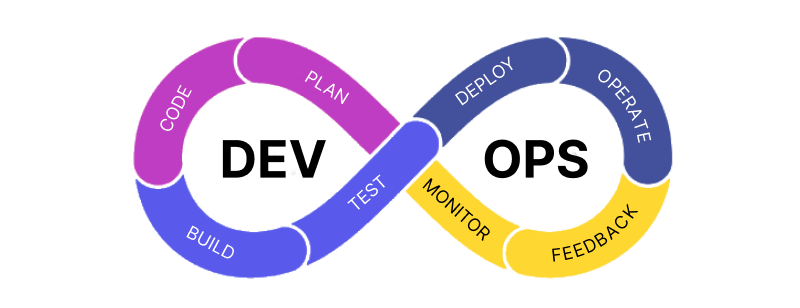
\includegraphics[width=0.75\textwidth]{assets/devops_cycle.png}
    \caption{Cycle de vie DevOps -- boucle d'amélioration continue (Source : \cite{katalon2024devops})}
    \label{fig:devops-cycle}
\end{figure}

Concrètement, les pratiques DevOps retenues pour RevMine se déclinent selon les différentes
étapes du cycle DevOps~:

\begin{itemize}
    \item \textbf{Planification (Plan)}~: définition des besoins fonctionnels et techniques du
          système, rédaction des exigences, organisation des tâches et planification des sprints
          selon la méthodologie Scrum~;

    \item \textbf{Développement (Code)}~: développement collaboratif sur GitLab avec gestion de
          versions et revue systématique des contributions via des Merge Requests~;

    \item \textbf{Construction (Build)}~: génération et construction automatisée des images Docker
          après chaque fusion sur la branche principale. Chaque service dispose de son propre
          \texttt{Dockerfile}~;

    \item \textbf{Tests (Test)}~: exécution automatique des tests unitaires, des tests
          d'intégration et des analyses de qualité statique via les pipelines GitLab CI à
          chaque commit~;

    \item \textbf{Déploiement (Deploy)}~: orchestration et déploiement des services applicatifs
          et d'infrastructure à l'aide de Docker Compose et du pipeline CI/CD GitLab~;

    \item \textbf{Exploitation (Operate)}~: gestion et exécution continue des services de la
          plateforme afin d'assurer leur disponibilité, leur stabilité et leur bon fonctionnement
          dans l'environnement de développement et de recherche~;

    \item \textbf{Retour d'expérience (Feedback)}~: collecte des retours de l'équipe de recherche
          de l'ETS ainsi que des utilisateurs métier afin d'améliorer les fonctionnalités,
          l'ergonomie et les performances du système~;

    \item \textbf{Surveillance (Monitor)}~: suivi des journaux applicatifs via la pile
          Grafana~+~Loki~+~Promtail, supervision des erreurs et observation des performances des
          services en temps réel.
\end{itemize}

Ce cycle est itératif~: les retours collectés durant les phases d'exploitation et de surveillance
permettent de revenir à l'étape de planification afin d'identifier de nouveaux besoins, corriger
les limitations observées et améliorer continuellement la plateforme RevMine.

% ============================================================
\section{Planification}
% ============================================================

\subsection{Méthodologie Scrum}

La gestion du projet s'est inspirée de la méthode \textbf{Scrum}, cadre agile structurant le
développement en itérations courtes et régulières appelées \textit{sprints}
\parencite{schwaber2020scrum}. Les sprints ont été fixés à une durée d'une semaine, permettant
des cycles de livraison rapides et une adaptation continue aux retours obtenus.

Le projet RevMine a été réalisé en \textbf{binôme}, ce qui a nécessité une coordination étroite
tout au long du développement. Deux cadences de réunion ont structuré le suivi du projet~:

\begin{itemize}
    \item \textbf{Réunions hebdomadaires (chaque jeudi)}~: ces séances servaient à la fois de
          revue de sprint et de planification. Nous y présentions les fonctionnalités développées
          au cours de la semaine, levions les blocages techniques et définissions les objectifs du
          sprint suivant. La régularité de ces rendez-vous a permis une adaptation rapide aux
          retours et un alignement continu entre les réalisations et les attentes du projet~;

    \item \textbf{Réunions mensuelles}~: à un rythme mensuel, l'équipe présentait l'avancement
          global du projet devant l'équipe de recherche de l'\textbf{ETS} (École de Technologie
          Supérieure). Ces réunions constituaient une opportunité précieuse d'obtenir un retour
          critique de la part de professionnels du métier, apportant un regard extérieur sur les
          choix fonctionnels et techniques de la plateforme. Les observations formulées lors de
          ces séances ont contribué à affiner certaines orientations du projet et à valider la
          pertinence des fonctionnalités développées au regard des besoins réels du terrain.
\end{itemize}

Cette double cadence de suivi -- hebdomadaire pour le pilotage opérationnel et mensuelle pour la
validation avec l'équipe de recherche -- a favorisé une livraison incrémentale des fonctionnalités
et une détection précoce des écarts tout au long du développement.

\subsection{Tableau Kanban}

La gestion des tâches a été assurée à l'aide du tableau \textbf{Kanban} (littéralement
\og{}panneau visuel\fg{} en japonais) intégré à GitLab. Cet outil offre une représentation
visuelle de l'état d'avancement de chaque tâche, permettant aux deux membres du binôme
d'identifier rapidement les blocages et de prioriser les efforts. Chaque fonctionnalité,
correction ou amélioration a été formalisée sous forme d'\textit{issue}, puis suivie tout au
long de son cycle de vie grâce à cinq statuts distincts et un système d'étiquettes structuré.

\subsubsection*{Statuts du tableau}

Cinq statuts ont été définis pour refléter fidèlement l'avancement de chaque tâche~:

\begin{itemize}
    \item \textbf{À faire} (\textit{To Do})~: la tâche est identifiée et planifiée pour le sprint
          en cours, mais le développement n'a pas encore débuté~;
    \item \textbf{En cours} (\textit{In Progress})~: le développement est actif~; une seule
          personne du binôme est responsable de la tâche à ce stade afin d'éviter les conflits
          de travail~;
    \item \textbf{En revue} (\textit{Under Review})~: le développement est terminé et une Merge
          Request a été ouverte~; la tâche est en attente de revue par l'autre membre du binôme
          avant intégration~;
    \item \textbf{Bloquée} (\textit{Blocked})~: la tâche ne peut pas avancer en raison d'une
          dépendance non résolue ou d'un blocage technique~; ce statut permet de signaler
          rapidement les obstacles et de les traiter en priorité lors des points hebdomadaires~;
    \item \textbf{Clôturée} (\textit{Closed})~: la tâche est terminée, revue, intégrée dans la
          branche principale et validée.
\end{itemize}

\subsubsection*{Système d'étiquettes}

Chaque issue est enrichie d'un ensemble d'étiquettes permettant de la caractériser selon plusieurs
dimensions~:

\begin{itemize}
    \item \textbf{Composant}~: \texttt{frontend}, \texttt{backend} ou \texttt{ai}, indiquant la
          couche technique concernée~;
    \item \textbf{Nature}~: \texttt{feat} (nouvelle fonctionnalité) ou \texttt{bug} (correction
          d'un défaut)~;
    \item \textbf{Priorité}~: niveau d'urgence parmi \texttt{low}, \texttt{medium} et
          \texttt{high}, facilitant l'arbitrage lors de la planification du sprint~;
    \item \textbf{Sprint}~: étiquette indiquant le sprint auquel la tâche est rattachée, assurant
          la traçabilité de la charge de travail par itération.
\end{itemize}

La Figure~\ref{fig:kanban} illustre le tableau Kanban tel qu'utilisé dans GitLab, avec les
différentes colonnes de statut et le système d'étiquettes.

\begin{figure}[H]
    \centering
    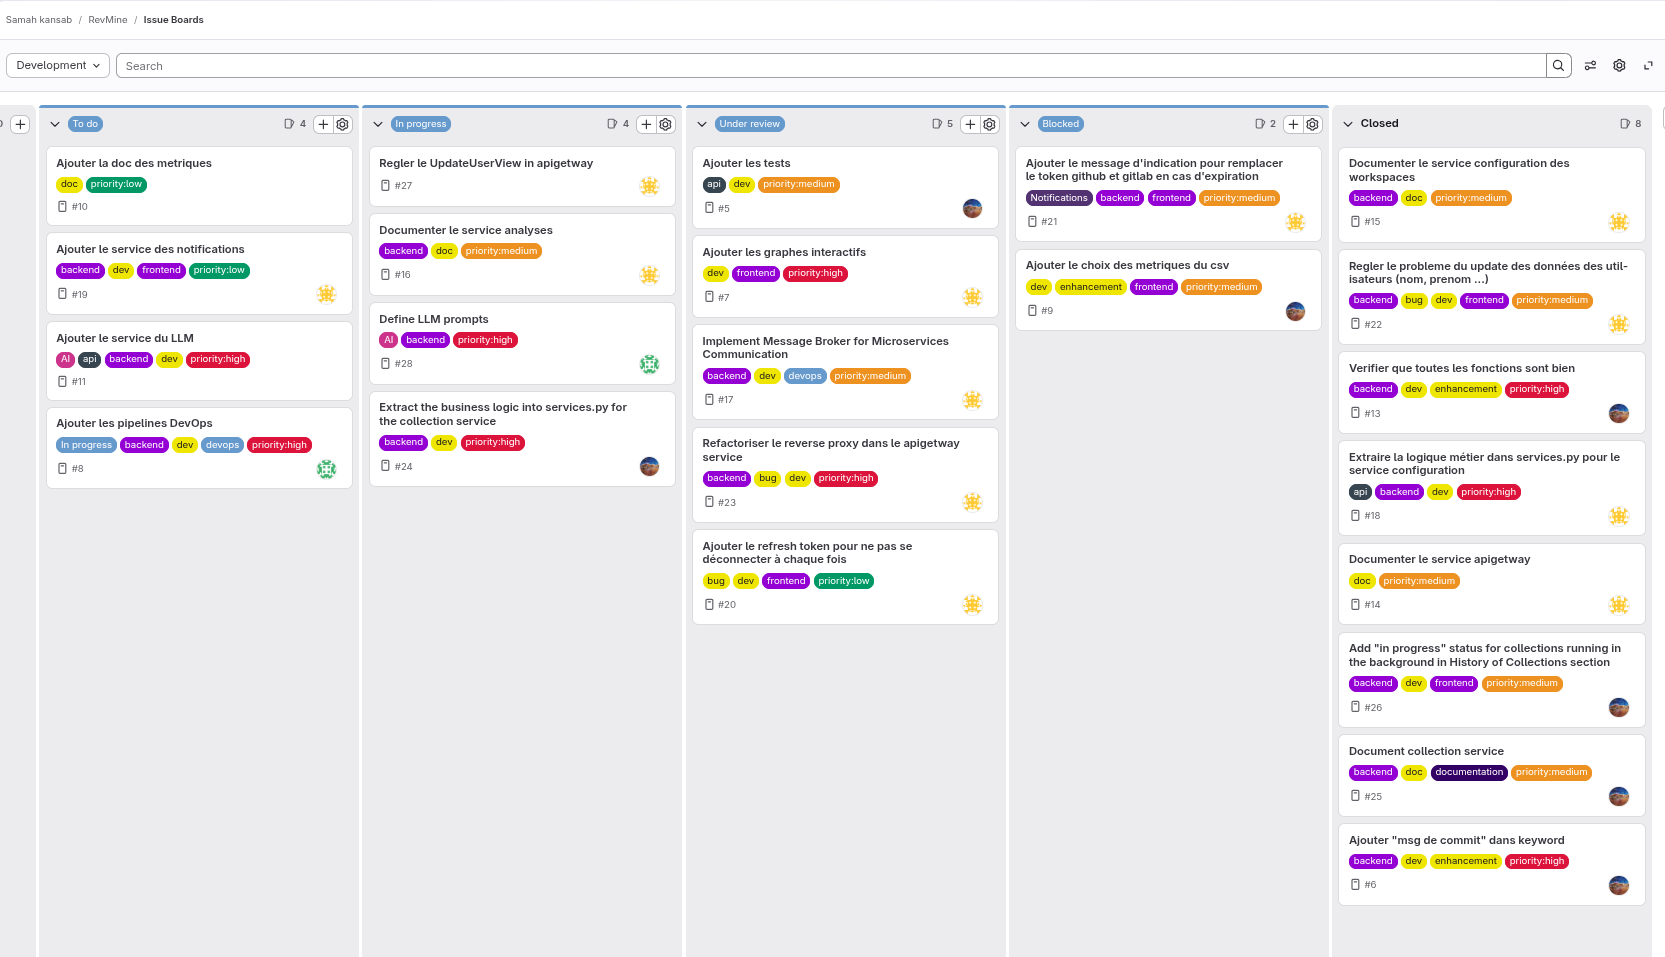
\includegraphics[width=0.95\textwidth]{captures/kanban_board.png}
    \caption{Tableau Kanban GitLab utilisé pour le suivi des tâches du projet RevMine}
    \label{fig:kanban}
\end{figure}

% ============================================================
\section{Développement}
% ============================================================

\subsection{Politique de gestion des branches}

Afin de maintenir la lisibilité de l'historique Git et de sécuriser l'intégrité de la branche
principale, une \textbf{politique de branches} rigoureuse a été adoptée, s'inspirant du
\textit{Feature Branch Workflow} \parencite{atlassian2023gitflow}. Ce modèle préconise que chaque
nouvelle unité de travail -- fonctionnalité, correction ou amélioration -- soit développée dans
une branche dédiée, isolant ainsi les modifications en cours des livrables stables.

\subsubsection*{Justification du choix}

Plusieurs alternatives ont été envisagées. Le modèle \textit{Gitflow} classique, avec ses branches
\texttt{develop}, \texttt{release} et \texttt{hotfix}, s'avère surdimensionné pour un binôme
réalisant des livraisons continues sans gestion de versions numérotées. Le \textit{Trunk-Based
Development}, où tous les développeurs poussent directement sur la branche principale, présente un
risque élevé d'instabilité pour un projet en construction active. Le \textit{Feature Branch
Workflow} représente le meilleur compromis~: chaque fonctionnalité est isolée dans sa propre
branche, ce qui protège la branche principale tout en restant simple à opérer à deux.

\subsubsection*{Convention de nommage}

La convention de nommage suivante a été appliquée de manière systématique~:

\begin{itemize}
    \item \texttt{feature/<nom-fonctionnalité>}~-- développement d'une nouvelle fonctionnalité~;
    \item \texttt{fix/<description-du-bug>}~-- correction d'un défaut~;
    \item \texttt{refactor/<module>}~-- refactorisation d'un composant existant~;
    \item \texttt{test/<service>}~-- ajout ou mise à jour de tests~;
    \item \texttt{docs/<sujet>}~-- modification de la documentation.
\end{itemize}

Ce nommage structuré présente plusieurs avantages~: il permet d'identifier instantanément la
nature et la portée d'une branche, facilite le filtrage et la recherche dans l'historique Git,
et réduit les risques de confusion lors des revues de code. Toutes les branches sont créées
depuis \texttt{main} et fusionnées après revue via une Merge Request. Aucun commit direct sur
la branche principale n'est autorisé, garantissant ainsi la stabilité permanente du code de
référence.

\subsection{Revue de code}

La branche \texttt{main} du dépôt GitLab a été configurée en mode \textbf{protégé}~: aucun
commit direct n'y est autorisé, et toute intégration passe obligatoirement par une
\textbf{Merge Request} (MR). Ce mécanisme constitue le point de contrôle central de la qualité
du code tout au long du développement.

Selon la nature et la portée de la tâche, deux niveaux de revue ont été appliqués~:

\begin{itemize}
    \item \textbf{Revue croisée}~: pour les fonctionnalités significatives, les modifications
          d'architecture ou les corrections de bugs critiques, la MR est soumise à l'examen de
          l'autre membre du binôme et, lorsque pertinent, à l'encadrant. La revue porte sur la
          correction fonctionnelle, la lisibilité du code, le respect des conventions de nommage
          et de structure, ainsi que l'absence de régressions. Les remarques sont formulées
          directement sous forme de commentaires inline dans GitLab, favorisant un échange précis
          et traçable~;
    \item \textbf{Auto-approbation}~: pour les tâches mineures -- corrections typographiques dans
          la documentation, ajustements de configuration, mises à jour de dépendances sans impact
          fonctionnel -- le membre ayant ouvert la MR procède lui-même à son approbation
          (\textit{self-approve}), afin de ne pas bloquer inutilement le flux de travail sur des
          changements à faible risque.
\end{itemize}

Cette politique à deux vitesses permet de concilier rigueur et agilité~: les modifications
sensibles bénéficient d'un regard extérieur systématique, tandis que les tâches routinières ne
génèrent pas de délais d'attente superflus. La Figure~\ref{fig:code-review} illustre un exemple
de revue de code réalisée sur une Merge Request, avec des commentaires formulés directement sur
les lignes concernées.

\begin{figure}[H]
    \centering
    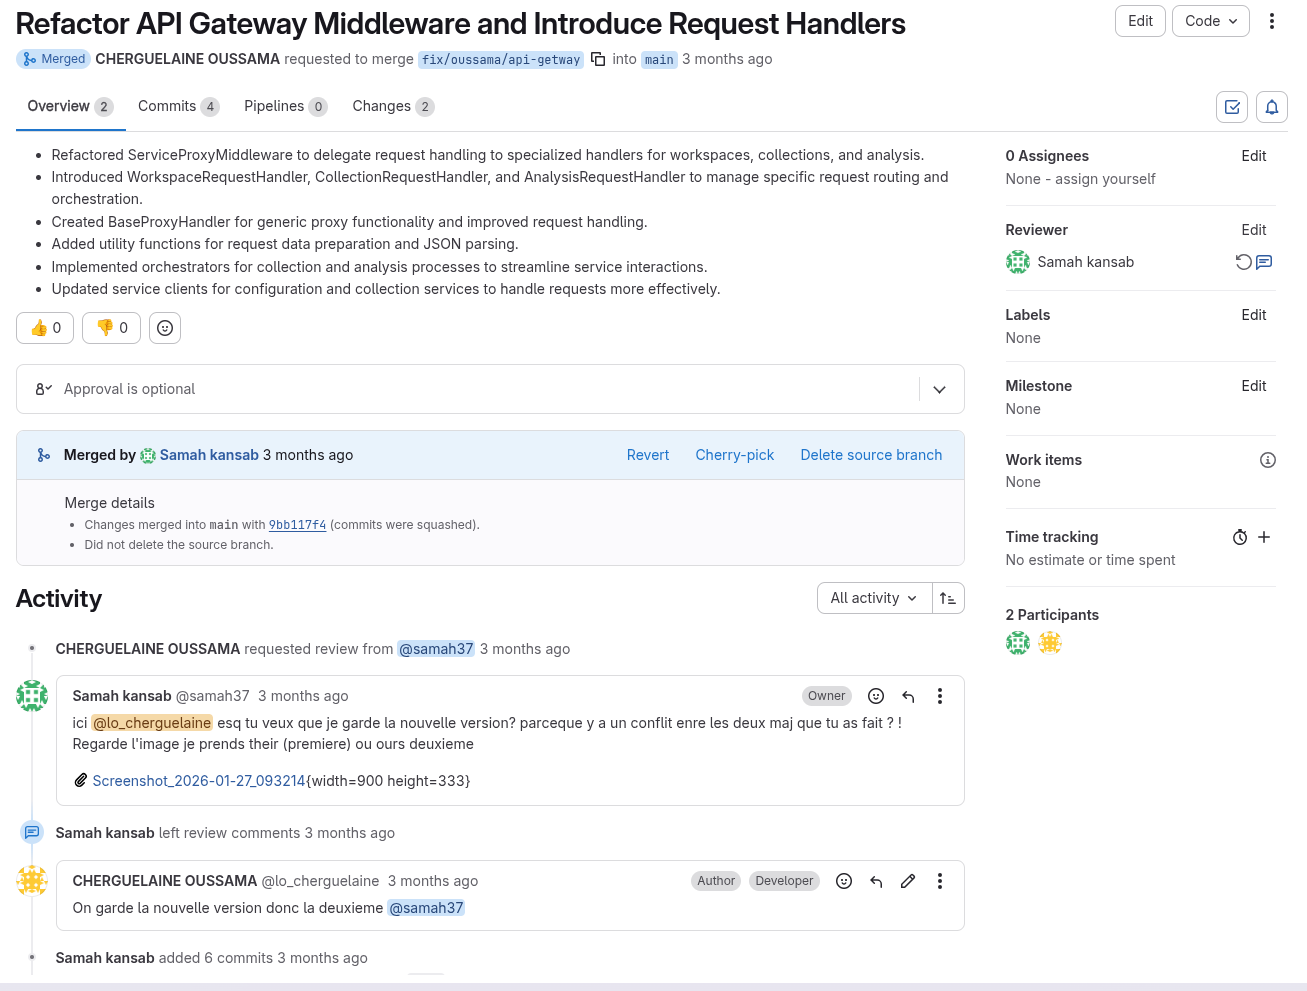
\includegraphics[width=0.95\textwidth]{captures/code_review.png}
    \caption{Exemple de revue de code sur une Merge Request GitLab dans le projet RevMine}
    \label{fig:code-review}
\end{figure}

\subsection{Réalisation du backend}

Le backend de RevMine est composé de plusieurs microservices spécialisés, chacun prenant en
charge un périmètre fonctionnel précis. Les sections suivantes détaillent l'implémentation de
chacun d'eux.

% ------------------------------------------------------------
\subsubsection{API Gateway}
% ------------------------------------------------------------

L'API Gateway constitue le point d'entrée unique de l'application. Développé avec
\textbf{Django} et \textbf{Django REST Framework}, il centralise l'authentification des
utilisateurs et orchestre les appels vers les services internes, évitant ainsi au frontend
d'avoir à connaître l'adresse de chaque microservice.

Ce service gère l'inscription, la connexion et la gestion du profil utilisateur. L'authentification
repose sur des \textbf{tokens JWT}\footnote{JWT (\textit{JSON Web Token})~: standard ouvert (RFC
7519) définissant un format compact et autonome pour la transmission sécurisée d'informations entre
parties sous forme d'objet JSON signé numériquement.}, avec prise en charge du rafraîchissement
de session par l'émission d'un \textit{refresh token} de longue durée. En complément de
l'authentification classique par email et mot de passe, le service intègre l'authentification
\textbf{OAuth}\footnote{OAuth (\textit{Open Authorization})~: protocole standard d'autorisation
permettant à une application d'accéder aux ressources d'un utilisateur chez un fournisseur tiers
sans que l'utilisateur n'ait à partager ses identifiants.} via GitHub, GitLab et Google,
simplifiant l'accès à la plateforme pour les développeurs.

La documentation interactive des API est générée automatiquement grâce à
\textbf{drf-spectacular}. Les principaux endpoints exposés par ce service sont détaillés dans
le tableau ci-après.

\begin{table}[H]
\centering
\small
\caption{Endpoints principaux de l'API Gateway}
\label{tab:endpoints-gateway}
\begin{tabular}{|>{\centering\arraybackslash}p{1.6cm}
                |>{\raggedright\arraybackslash}p{6.2cm}
                |>{\raggedright\arraybackslash}p{4.8cm}|}
\hline
\textbf{Méthode} & \textbf{Route} & \textbf{Description} \\
\hline
POST & \texttt{/api/auth/register} & Inscription d'un nouvel utilisateur \\
\hline
POST & \texttt{/api/auth/login} & Authentification par email et mot de passe \\
\hline
POST & \texttt{/api/auth/refresh} & Renouvellement du token JWT \\
\hline
GET & \texttt{/api/auth/me} & Profil de l'utilisateur connecté \\
\hline
PATCH & \texttt{/api/auth/me/update/} & Mise à jour des informations du profil \\
\hline
POST & \texttt{/api/auth/me/change-password/} & Changement de mot de passe \\
\hline
DELETE & \texttt{/api/auth/me/delete/} & Suppression du compte utilisateur \\
\hline
GET / POST & \texttt{/api/auth/oauth/github} & Authentification OAuth via GitHub \\
\hline
GET / POST & \texttt{/api/auth/oauth/gitlab} & Authentification OAuth via GitLab \\
\hline
GET / POST & \texttt{/api/auth/oauth/google} & Authentification OAuth via Google \\
\hline
GET & \texttt{/api/docs/} & Documentation Swagger interactive \\
\hline
\end{tabular}
\end{table}

% ------------------------------------------------------------
\subsubsection{Service de configuration}
% ------------------------------------------------------------

Le service de configuration gère les \textit{workspaces} et les dépôts associés. Il permet à
l'utilisateur de créer un espace de travail, de spécifier la plateforme cible (GitHub ou GitLab),
de fournir un jeton d'accès\footnote{Un jeton d'accès (\textit{access token}) est une clé secrète
générée par une plateforme permettant à une application tierce d'interagir avec son API au nom de
l'utilisateur, sans exposer les identifiants de connexion.} et de valider la connexion. Une fois
la connexion établie, le service interroge la plateforme distante pour récupérer la liste des
dépôts disponibles, que l'utilisateur peut ensuite importer dans son espace local.

La séparation entre la gestion des sources de données et les traitements analytiques améliore la
maintenabilité de l'ensemble et facilite l'évolution indépendante de chaque composant. Les
endpoints de ce service sont répertoriés dans le tableau suivant.

\begin{table}[H]
\centering
\small
\caption{Endpoints principaux du service de configuration}
\label{tab:endpoints-config}
\begin{tabular}{|>{\centering\arraybackslash}p{2cm}
                |>{\raggedright\arraybackslash}p{7cm}
                |>{\raggedright\arraybackslash}p{3.5cm}|}
\hline
\textbf{Méthode} & \textbf{Route} & \textbf{Description} \\
\hline
GET / POST & \texttt{/api/workspaces/} & Liste et création de workspaces \\
\hline
GET / PUT / DELETE & \texttt{/api/workspaces/<id>/} & Lecture, mise à jour, suppression \\
\hline
GET & \texttt{/api/workspaces/<id>/token/} & Récupération du token chiffré \\
\hline
POST & \texttt{/api/workspaces/test/} & Test de connexion à la plateforme \\
\hline
GET & \makecell[l]{\texttt{/api/workspaces/<id>/} \\ \texttt{remote-repositories/}} & Dépôts distants disponibles \\
\hline
POST & \makecell[l]{\texttt{/api/workspaces/<id>/} \\ \texttt{repositories/import/}} & Import local des dépôts sélectionnés \\
\hline
GET & \texttt{/api/workspaces/<id>/repositories/} & Liste des dépôts importés \\
\hline
DELETE & \makecell[l]{\texttt{/api/workspaces/<id>/} \\ \texttt{repositories/<repo\_id>/}} & Suppression d'un dépôt importé \\
\hline
GET & \texttt{/api/workspaces/repositories/all/} & Liste globale de tous les dépôts \\
\hline
\end{tabular}
\end{table}

% ------------------------------------------------------------
\subsubsection{Service de collecte}
% ------------------------------------------------------------

Le service de collecte est l'un des modules centraux de RevMine. Il récupère les données issues
des plateformes de développement -- notamment les \textit{merge requests}, \textit{pull requests},
branches et métadonnées associées depuis GitHub et GitLab -- selon un \textbf{workflow progressif}
structuré en six étapes~:

\begin{enumerate}
    \item sélection du dépôt à traiter~;
    \item récupération des branches disponibles~;
    \item sélection des métriques à collecter~;
    \item validation du plan de collecte~;
    \item exécution, suspension ou reprise de la collecte~;
    \item consultation des résultats.
\end{enumerate}

Ce service prend également en charge l'\textbf{importation de collections externes} au format
JSON, permettant d'intégrer des données déjà exportées depuis d'autres sources. Les données brutes
collectées sont archivées dans \textbf{MinIO}, tandis que les métadonnées de suivi sont conservées
en base relationnelle.

Une étape de \textbf{nettoyage et de structuration} transforme ensuite les données brutes en
fichiers CSV exploitables, prêts pour l'analyse. Cette séparation entre collecte et préparation
des données garantit la traçabilité et facilite la réutilisation des jeux de données. Le tableau
ci-dessous liste les endpoints exposés par ce service.

\begin{table}[H]
\centering
\small
\caption{Endpoints principaux du service de collecte}
\label{tab:endpoints-collection}
\begin{tabular}{|>{\centering\arraybackslash}p{1.5cm}
                |>{\raggedright\arraybackslash}p{7.2cm}
                |>{\raggedright\arraybackslash}p{3.8cm}|}
\hline
\textbf{Méthode} & \textbf{Route} & \textbf{Description} \\
\hline
POST & \texttt{/api/collections/start/} & Initialisation d'un plan de collecte \\
\hline
POST & \makecell[l]{\texttt{/api/collections/plans/<id>/} \\ \texttt{configure/}} & Sélection des métriques \\
\hline
POST & \makecell[l]{\texttt{/api/collections/plans/<id>/} \\ \texttt{validate/}} & Validation du plan de collecte \\
\hline
POST & \makecell[l]{\texttt{/api/collections/plans/<id>/} \\ \texttt{execute/}} & Lancement de la collecte \\
\hline
GET & \makecell[l]{\texttt{/api/collections/plans/<id>/} \\ \texttt{status/}} & Suivi de la progression \\
\hline
POST & \makecell[l]{\texttt{/api/collections/plans/<id>/} \\ \texttt{pause/}} & Suspension de la collecte \\
\hline
POST & \makecell[l]{\texttt{/api/collections/plans/<id>/} \\ \texttt{resume/}} & Reprise d'une collecte suspendue \\
\hline
POST & \makecell[l]{\texttt{/api/collections/plans/<id>/} \\ \texttt{apply-filters/}} & Filtres et génération du CSV \\
\hline
GET & \makecell[l]{\texttt{/api/collections/cleaned-data/} \\ \texttt{<id>/download/<type>/}} & Téléchargement du CSV généré \\
\hline
POST & \texttt{/api/collections/upload-external/} & Import d'une collection externe \\
\hline
\end{tabular}
\end{table}

% ------------------------------------------------------------
\subsubsection{Service d'analyse}
% ------------------------------------------------------------

Le service d'analyse transforme les datasets préparés en résultats analytiques et visuels. Il
permet d'importer des datasets, d'afficher un aperçu des colonnes disponibles, d'identifier
automatiquement les métriques compatibles et de générer des graphiques correspondants.

Pour gérer les traitements potentiellement coûteux en temps, le service s'appuie sur
\textbf{Celery} pour l'exécution asynchrone des tâches et sur \textbf{Redis} comme broker de
messages. Cette architecture permet à l'interface utilisateur de rester réactive pendant
l'exécution des calculs, notamment lors de l'analyse de jeux de données volumineux ou de la
génération de plusieurs visualisations en parallèle. Les analyses réalisées sont sauvegardées
et consultables via un historique. Le cycle de vie complet d'une analyse est couvert par les
endpoints répertoriés dans le tableau suivant.

\begin{table}[H]
\centering
\small
\caption{Endpoints principaux du service d'analyse}
\label{tab:endpoints-analyze}
\begin{tabular}{|>{\centering\arraybackslash}p{1.5cm}
                |>{\raggedright\arraybackslash}p{7.2cm}
                |>{\raggedright\arraybackslash}p{3.8cm}|}
\hline
\textbf{Méthode} & \textbf{Route} & \textbf{Description} \\
\hline
POST & \texttt{/api/analysis/datasets/upload/} & Import d'un dataset (CSV) \\
\hline
GET & \texttt{/api/analysis/datasets/<id>/columns/} & Colonnes et types disponibles \\
\hline
GET & \texttt{/api/analysis/datasets/<id>/preview/} & Aperçu des premières lignes \\
\hline
GET & \makecell[l]{\texttt{/api/analysis/datasets/<id>/} \\ \texttt{available\_metrics/}} & Métriques compatibles \\
\hline
POST & \texttt{/api/analysis/generate/} & Génération d'un graphique \\
\hline
GET & \texttt{/api/analysis/analyses/} & Historique des analyses réalisées \\
\hline
POST & \texttt{/api/analysis/analyses/bulk\_create/} & Création de plusieurs analyses \\
\hline
GET & \texttt{/api/analysis/analyses/<id>/result/} & Résultat et image du graphique \\
\hline
POST & \texttt{/api/analysis/analyses/<id>/retry/} & Relance d'une analyse existante \\
\hline
GET & \texttt{/api/analysis/metrics/} & Catalogue des métriques disponibles \\
\hline
\end{tabular}
\end{table}

% ------------------------------------------------------------
\subsubsection{Service d'intelligence artificielle (LLM)}
\label{subsec:service-llm}
% ------------------------------------------------------------

RevMine intègre un service dédié au traitement du langage naturel, développé avec
\textbf{FastAPI}. Ce service constitue l'interface entre l'utilisateur et les modèles de
langage~: il interprète des requêtes formulées en langage naturel -- telles que \og{}Analyse les
données des six derniers mois sur la branche principale\fg{} -- et les transforme en plans de
collecte ou d'analyse structurés, directement exécutables par les autres services de la
plateforme.

\subsubsection*{Architecture du service}

Le service LLM est architecturé comme un microservice \textbf{sans état} (\textit{stateless}),
exposant deux endpoints distincts selon le fournisseur de modèle~: \texttt{/ollama} pour
l'inférence locale et \texttt{/openrouter} pour les modèles hébergés. Cette conception lui
confère une scalabilité horizontale native, sans modification de l'architecture lors d'une montée
en charge.

L'intégration avec l'API Gateway s'effectue via HTTP REST. Lorsqu'un utilisateur active le mode
automatique depuis l'interface, l'API Gateway délègue la requête à l'orchestrateur correspondant
(\texttt{CollectionOrchestrator} ou \texttt{AnalysisOrchestrator}), qui exécute le pipeline de
traitement suivant~:

\begin{enumerate}
    \item Récupération des métadonnées du dépôt ciblé auprès du service de configuration~;
    \item Construction d'un prompt contextualisé enrichi de ces métadonnées (identifiant,
          plateforme, nom du dépôt) et de la requête en langage naturel de l'utilisateur~;
    \item Transmission au service LLM via l'endpoint \texttt{/openrouter} ou \texttt{/ollama}
          selon le mode sélectionné~;
    \item Réception du plan structuré JSON, normalisation et validation des dépendances de
          métriques par la fonction \texttt{normalize\_collection\_automation\_payload()}~;
    \item Retour du plan validé au frontend pour confirmation utilisateur avant exécution.
\end{enumerate}

Côté service LLM, chaque requête est traitée selon la séquence interne suivante~: le prompt
système est construit dynamiquement via \texttt{build\_system\_prompt()} avec injection de la
date courante (\texttt{\_\_TODAY\_\_})~; la paire (prompt système, message utilisateur) est
soumise au modèle avec une température fixée à \textbf{0} pour maximiser le déterminisme des
sorties~; enfin, la réponse brute est traitée par \texttt{extract\_json\_object()} qui tente
d'abord un décodage JSON direct, puis une extraction par expression régulière en cas de texte
enveloppant le JSON.

\begin{table}[H]
\centering
\small
\caption{Endpoints du service LLM (FastAPI)}
\label{tab:endpoints-llm}
\begin{tabular}{|>{\centering\arraybackslash}p{1.5cm}
                |>{\raggedright\arraybackslash}p{4.5cm}
                |>{\raggedright\arraybackslash}p{6.5cm}|}
\hline
\textbf{Méthode} & \textbf{Route} & \textbf{Description} \\
\hline
GET & \texttt{/health} & Vérification de l'état du service \\
\hline
GET & \texttt{/models} & Liste des fournisseurs et modèles disponibles \\
\hline
POST & \texttt{/ollama} & Traitement via Ollama (inférence locale) \\
\hline
POST & \texttt{/openrouter} & Traitement via OpenRouter (hébergé) \\
\hline
\end{tabular}
\end{table}

\subsubsection*{Ingénierie des prompts par consensus~: le processus NGT}
\label{subsubsec:ngt}

La conception du service repose sur une \textbf{ingénierie de prompts}\footnote{\textit{Prompt
engineering}~: discipline consistant à concevoir et structurer les instructions transmises à un
modèle de langage afin de maximiser la pertinence, la fiabilité et la conformité de ses réponses.}
structurée. Dans le contexte de RevMine, la qualité du prompt n'est pas uniquement une question
de style~: un prompt incomplet ou mal structuré peut produire des noms de métriques invalides,
des dépendances manquantes, des filtres incorrects ou des sorties JSON malformées, chacun de ces
défauts compromettant la correction ou l'exécutabilité du plan de collecte généré.

Afin de garantir un processus de conception rigoureux et traçable, un processus inspiré de la
\textbf{Technique du Groupe Nominal} (\textit{Nominal Group Technique}, NGT) a été adopté
\parencite{mcmillan2016ngt, rileybennett2024ngt}. La NGT est une méthode de construction de
consensus qui combine une génération d'idées indépendante et une discussion structurée ultérieure,
réduisant ainsi les biais d'ancrage et d'influence entre participants. Ce processus se déroule en
quatre étapes, résumées dans la Figure~\ref{fig:ngt-process}.

\begin{figure}[H]
    \centering
    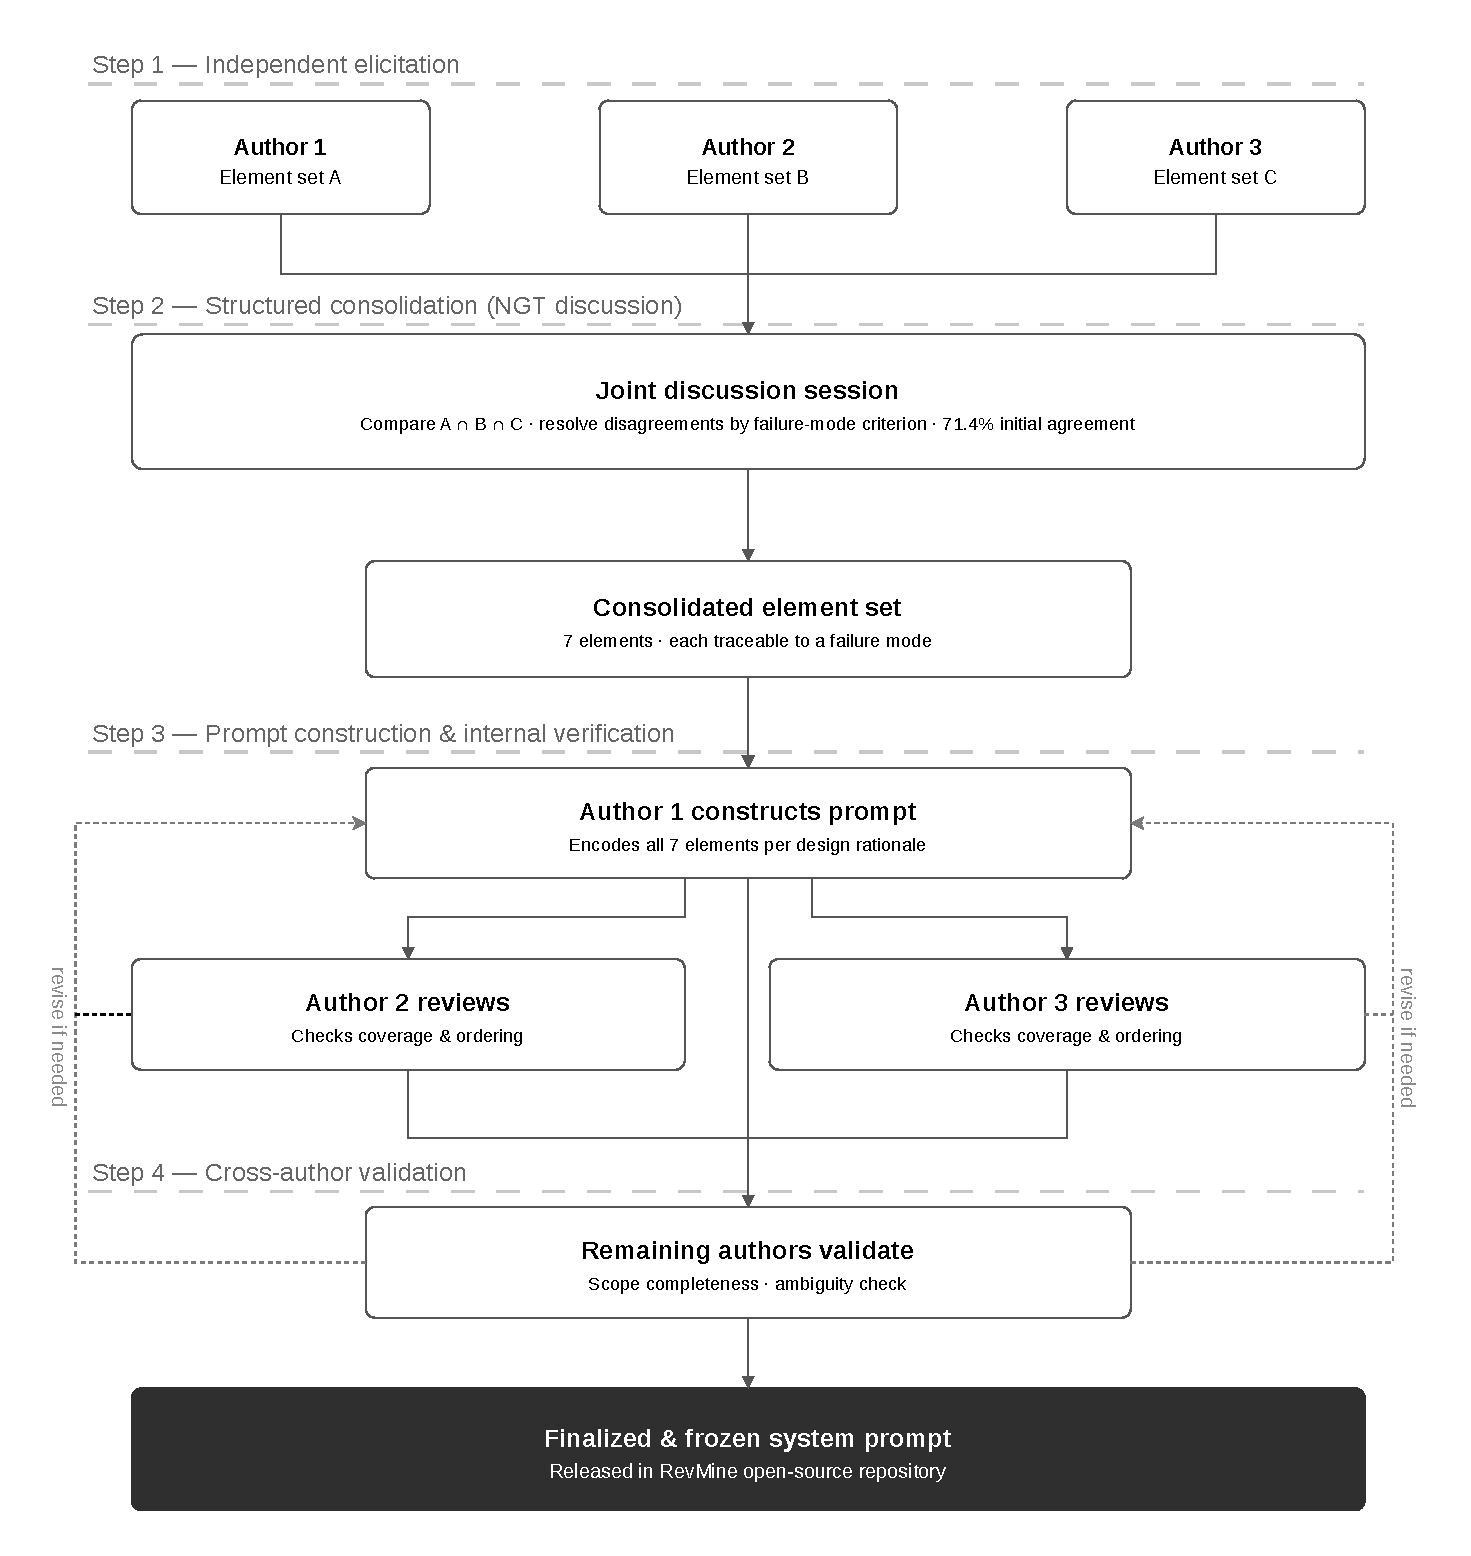
\includegraphics[width=\textwidth]{assets/ngt_revmine_diagram.pdf}
    \caption{Vue d'ensemble du processus d'ingénierie de prompts basé sur la NGT modifiée}
    \label{fig:ngt-process}
\end{figure}

\begin{enumerate}
    \item \textbf{Élicitation indépendante.} Chaque auteur identifie indépendamment les éléments
          du prompt jugés nécessaires pour l'orchestration, en utilisant le mode de configuration
          manuelle de RevMine comme spécification de référence.

    \item \textbf{Consolidation structurée.} Les ensembles produits indépendamment sont comparés
          lors d'une session de discussion structurée. Les éléments proposés ne sont retenus que
          s'ils permettent de prévenir un mode de défaillance identifié.

    \item \textbf{Construction du prompt et vérification interne.} Un auteur construit le prompt
          système à partir des décisions de conception consolidées, puis le prompt résultant est
          examiné indépendamment par les autres auteurs.

    \item \textbf{Validation croisée.} Le prompt est soumis à une passe de validation finale par
          l'ensemble des auteurs afin de confirmer qu'il reflète fidèlement le périmètre
          opérationnel complet de RevMine.
\end{enumerate}

\subsubsection*{Éléments du prompt et modes de défaillance prévenus}

Sept éléments fondamentaux ont été intégrés au prompt système à l'issue du processus NGT. Le
Tableau~\ref{tab:prompt_elements_fr} les récapitule avec les modes de défaillance correspondants.

\begin{table}[H]
\centering
\small
\caption{Éléments du prompt système et modes de défaillance prévenus}
\label{tab:prompt_elements_fr}
\begin{tabular}{|>{\raggedright\arraybackslash}p{6.5cm}
                |>{\raggedright\arraybackslash}p{6.5cm}|}
\hline
\textbf{Élément du prompt} & \textbf{Mode de défaillance prévenu} \\
\hline
Énumération fermée de toutes les métriques valides & Hallucination de noms de métriques \\
\hline
Table de dépendances métriques\,/\,features & Omission de dépendances \\
\hline
Règles de classification de l'intention & Mauvaise classification de l'intention \\
\hline
Indicateurs de détection de la plateforme & Confusion GitHub\,/\,GitLab \\
\hline
Injection dynamique de la date courante (\texttt{\_\_TODAY\_\_}) & Mauvaise résolution des expressions temporelles \\
\hline
Règles de peuplement des filtres & Filtres incorrects ou manquants \\
\hline
Instruction de discipline de sortie stricte & JSON mal formé ou encadré de texte \\
\hline
\end{tabular}
\end{table}

\subsubsection*{Modes d'exécution~: inférence locale et inférence hébergée}

Le service LLM est conçu comme \textbf{agnostique au modèle}~: la couche d'orchestration
interagit avec les LLM via une interface unifiée, permettant de substituer différents backends
sans modifier la structure du prompt ni la logique de parsing en aval.

\paragraph{Mode Ollama -- inférence locale.} Ollama est un moteur d'inférence locale permettant
d'exécuter des modèles open source (Mistral, LLaMA, Gemma, etc.) directement sur la machine hôte,
sans dépendance à un service cloud \parencite{ollama2023}. Ce mode garantit la confidentialité
totale des données et l'absence de coût par requête, au prix de performances limitées par les
ressources locales disponibles.

\paragraph{Mode OpenRouter -- modèles hébergés.} OpenRouter est une passerelle d'API agrégeant
de nombreux fournisseurs de LLM (OpenAI, Anthropic, Google, Meta, etc.) sous une interface
unifiée compatible avec l'API OpenAI \parencite{openrouter2023}. Ce mode donne accès à des
modèles de grande capacité sans infrastructure GPU requise.

Le Tableau~\ref{tab:backend_modes_fr} synthétise les compromis pratiques entre les deux modes.

\begin{table}[H]
\centering
\small
\caption{Comparaison des deux modes d'exécution du service LLM de RevMine}
\label{tab:backend_modes_fr}
\begin{tabular}{|>{\raggedright\arraybackslash}p{3.5cm}
                |>{\raggedright\arraybackslash}p{5.5cm}
                |>{\raggedright\arraybackslash}p{5.5cm}|}
\hline
\textbf{Dimension} & \textbf{Ollama (local)} & \textbf{OpenRouter (hébergé)} \\
\hline
Traitement des données & Les requêtes restent sur la machine locale & Les requêtes sont transmises à un fournisseur externe \\
\hline
Infrastructure requise & Environnement local et poids du modèle téléchargés & Connexion Internet et clé API \\
\hline
Accès aux modèles & Limité aux modèles exécutables localement & Large accès aux modèles commerciaux et open-weight \\
\hline
Confidentialité & Contrôle local fort des données & Soumis aux politiques du fournisseur externe \\
\hline
Reproductibilité & Élevée si la version du modèle est figée & Dépend de la stabilité de la version distante \\
\hline
Structure de coût & Pas de facturation par requête~; coût matériel local & Options gratuites et payantes selon le modèle \\
\hline
\end{tabular}
\end{table}

% ------------------------------------------------------------
\subsubsection{Service de notification}
% ------------------------------------------------------------

Le service de notification a été développé en \textbf{Go} avec le framework \textbf{Fiber}. Ce
choix répond à la nécessité de gérer un grand nombre de connexions WebSocket concurrentes avec
une faible empreinte mémoire, exigence difficile à satisfaire avec des frameworks synchrones
traditionnels.

Ce service consomme les événements publiés sur Kafka par les autres services, les persiste dans
sa propre base PostgreSQL, puis les diffuse en temps réel aux clients connectés via WebSocket.
L'utilisateur reçoit ainsi instantanément des informations sur l'état d'une collecte, la fin
d'un traitement ou toute anomalie survenue. Des endpoints complémentaires permettent de lister
les notifications, de comptabiliser les éléments non lus, de les marquer comme lus ou de les
supprimer.

% ============================================================
\subsection{Gestion des données et communication inter-services}
% ============================================================

La cohérence globale de RevMine repose sur une stratégie claire de gestion des données. Chaque
microservice dispose de sa propre base \textbf{PostgreSQL}, garantissant l'isolation des
responsabilités et limitant les dépendances directes entre services -- principe fondateur de
l'architecture microservices.

Les données brutes issues de la collecte sont archivées dans \textbf{MinIO} au format JSON,
séparant ainsi les artefacts bruts du stockage relationnel et facilitant leur réutilisation sans
relancer les appels API vers les plateformes distantes.

La communication entre services s'articule autour de deux mécanismes complémentaires~:

\begin{itemize}
    \item les \textbf{API REST}, pour les interactions synchrones initiées par le frontend ou
          l'API Gateway, lorsqu'une réponse immédiate est attendue~;
    \item \textbf{Apache Kafka}, comme bus de messages pour la communication asynchrone et le
          découplage des traitements internes, notamment pour les opérations longues telles que
          la collecte ou l'analyse de données.
\end{itemize}

Ces topics permettent, par exemple, au service de collecte d'informer le service d'analyse et
le service de notification de la disponibilité de nouvelles données, sans aucun couplage direct
entre eux. Le Tableau~\ref{tab:kafka-topics} détaille les topics Kafka utilisés dans la
plateforme, ainsi que leurs producteurs et consommateurs respectifs.

\begin{table}[H]
\centering
\small
\caption{Topics Kafka et flux de messages dans RevMine}
\label{tab:kafka-topics}
\begin{tabular}{|>{\raggedright\arraybackslash}p{6.2cm}
                |>{\raggedright\arraybackslash}p{3cm}
                |>{\raggedright\arraybackslash}p{3.5cm}|}
\hline
\textbf{Topic} & \textbf{Producteur} & \textbf{Consommateur(s)} \\
\hline
\texttt{config.tokens.request} & Collecte / Analyse & Configuration \\
\hline
\texttt{config.tokens.response} & Configuration & Collecte / Analyse \\
\hline
\texttt{collection.events.started} & Collecte & Notification \\
\hline
\texttt{collection.events.completed} & Collecte & Analyse, Notification \\
\hline
\texttt{collection.events.failed} & Collecte & Notification \\
\hline
\texttt{analysis.events.requested} & Analyse & Analyse \\
\hline
\texttt{analysis.events.completed} & Analyse & Notification \\
\hline
\texttt{notification.events} & Tous les services & Notification \\
\hline
\end{tabular}
\end{table}

% ============================================================
\subsection{Réalisation du frontend}
% ============================================================

Le frontend de RevMine a été développé sous la forme d'une \textbf{Single Page Application}
(SPA)\footnote{SPA (\textit{Single Page Application})~: application web qui charge une seule
page HTML au démarrage et met à jour dynamiquement le contenu sans rechargement complet de la
page, offrant une expérience utilisateur proche d'une application native.} avec \textbf{React},
offrant une navigation fluide entre les fonctionnalités.

\subsubsection{Structure générale de l'interface}

La navigation est assurée par \textbf{React Router} et les vues sont organisées en pages
fonctionnelles~: authentification, gestion des workspaces, gestion des projets, collecte et
nettoyage des données, analyse, profil et paramètres. Des \textit{layouts} distincts délimitent
les espaces accessibles sans authentification et les pages réservées aux utilisateurs connectés.

\subsubsection{Gestion de l'authentification et de l'état global}

L'authentification est centralisée dans des \textit{providers} React. Lors de la connexion, les
tokens JWT sont stockés côté client et automatiquement injectés dans les en-têtes des requêtes
HTTP via des \textbf{intercepteurs Axios}. Un mécanisme de rafraîchissement silencieux évite toute
interruption de session en cas d'expiration du token d'accès. La protection des routes garantit
que les pages sensibles sont inaccessibles aux utilisateurs non authentifiés.

\subsubsection{Modules fonctionnels}

\paragraph{Gestion des workspaces et des projets.} Ce module permet à l'utilisateur de créer et
gérer ses espaces de travail, de tester la connexion à une plateforme distante et d'importer les
dépôts souhaités. L'organisation par workspace puis par dépôt reflète le processus naturel de
travail dans un environnement de développement collaboratif.

\paragraph{Collecte et nettoyage des données.} L'interface de collecte guide l'utilisateur à
travers les étapes de configuration du plan de collecte~: sélection des branches, des métriques
et des filtres. Des écrans dédiés permettent de suivre la progression de l'exécution et de
consulter les résultats. Une fois les données récupérées, des vues spécifiques donnent accès au
nettoyage, à la génération de fichiers CSV structurés et à la consultation des jeux de données
préparés.

\paragraph{Analyse et visualisation.} Le module d'analyse constitue l'une des fonctionnalités
centrales de RevMine. Il permet de lancer une analyse à partir d'un fichier CSV ou d'un dataset
préparé, de sélectionner les métriques disponibles et de générer des représentations graphiques
adaptées au contenu des données. L'interface propose également un historique des analyses et un
tableau de bord analytique. Les visualisations sont produites avec \textbf{ECharts}, une
bibliothèque graphique offrant des représentations riches et interactives.

\subsubsection{Aspects ergonomiques et visuels}

L'interface repose sur \textbf{Tailwind CSS}, qui assure la cohérence des composants, des
espacements et des couleurs, tout en garantissant un comportement adaptatif sur différentes
tailles d'écran. L'organisation modulaire des composants React et l'utilisation de contextes
partagés contribuent à la maintenabilité du code frontend.

% ============================================================
\subsection{Sécurité de la solution}
% ============================================================

La sécurité a été intégrée dès la phase de conception, selon le principe du
\textit{security by design}. Les mécanismes de protection couvrent l'ensemble des couches de
la plateforme~: API Gateway, microservices internes, stockage des secrets et interface frontend.

\subsubsection{Authentification centralisée via l'API Gateway}

L'architecture de sécurité de RevMine repose sur un principe fondamental~: la
\textbf{centralisation de l'authentification au niveau de l'API Gateway}. Aucun microservice
interne n'est directement exposé à l'extérieur~; toutes les requêtes passent obligatoirement
par l'API Gateway, constituant le seul point d'entrée du système.

Le flux d'une requête authentifiée se déroule en quatre étapes, décrites dans le
Tableau~\ref{tab:flux-auth}~:

\begin{table}[H]
\centering
\small
\caption{Flux d'une requête authentifiée dans RevMine}
\label{tab:flux-auth}
\begin{tabular}{|>{\centering\arraybackslash}p{0.8cm}
                |>{\raggedright\arraybackslash}p{12.5cm}|}
\hline
\textbf{Étape} & \textbf{Description} \\
\hline
1 & Le frontend envoie la requête avec l'en-tête \texttt{Authorization: Bearer <token>} \\
\hline
2 & L'API Gateway extrait et valide le token JWT via \texttt{extract\_user\_from\_request()}~;
    en cas d'échec, une réponse \texttt{401 Unauthorized} est retournée immédiatement \\
\hline
3 & L'identifiant utilisateur (\texttt{user\_id}) est ajouté à la requête sous la forme
    d'un en-tête \texttt{X-User-ID} avant transmission au microservice cible \\
\hline
4 & Le microservice destinataire consomme uniquement cet en-tête \texttt{X-User-ID} pour
    associer les ressources à l'utilisateur, sans jamais accéder au token JWT \\
\hline
\end{tabular}
\end{table}

\subsubsection{Cycle de vie des tokens JWT}

L'authentification repose sur des \textbf{tokens JWT} (RFC~7519), gérés par la bibliothèque
\textbf{django-rest-framework-simplejwt}. À l'issue d'une authentification réussie, le service
génère~: un \textbf{token d'accès} d'une durée de vie de \textbf{60~minutes}, signé avec
l'algorithme HMAC-SHA256~; et un \textbf{token de rafraîchissement} valide pendant
\textbf{7~jours}, permettant d'obtenir silencieusement un nouveau token d'accès sans
ré-authentification.

\subsubsection{Chiffrement des tokens de plateformes tierces}

Les tokens d'accès personnels fournis par l'utilisateur pour s'authentifier auprès de GitHub ou
GitLab sont chiffrés avant stockage en base de données, en utilisant l'algorithme de chiffrement
symétrique \textbf{AES-128} via l'implémentation \textbf{Fernet} de la bibliothèque Python
\texttt{cryptography}. La clé de chiffrement est conservée comme variable d'environnement,
séparée du code source et exclue du dépôt.

\subsubsection{Mécanismes de sécurité complémentaires}

Plusieurs mécanismes complémentaires renforcent la posture de sécurité globale~:
\begin{itemize}
    \item \textbf{Middlewares Django}~: \texttt{SecurityMiddleware}, \texttt{XFrameOptionsMiddleware}
          et \texttt{CsrfViewMiddleware}~;
    \item \textbf{CORS}~: les origines autorisées sont configurées via
          \texttt{CORS\_ALLOWED\_ORIGINS}~;
    \item \textbf{Validation des mots de passe}~: quatre validateurs cumulatifs (similarité au
          profil, longueur minimale, mots de passe courants, refus des mots de passe numériques)~;
    \item \textbf{Gestion des secrets par variables d'environnement}~: toutes les clés sensibles
          sont chargées via \texttt{python-decouple} depuis un fichier \texttt{.env} exclu du
          dépôt~;
    \item \textbf{Isolation des bases de données}~: chaque microservice dispose de sa propre
          instance PostgreSQL~;
    \item \textbf{Timeouts des appels proxy}~: 300~s pour les requêtes standard, 1\,800~s pour
          les uploads.
\end{itemize}

% ============================================================
\section{Build}
\label{sec:build}
% ============================================================

La phase de build constitue l'étape qui transforme le code source validé en images Docker
autonomes et déployables. Dans RevMine, chaque microservice est empaquetté dans sa propre image,
garantissant l'isolation des dépendances et la reproductibilité des environnements entre le
développement, les tests et la production.

\subsection{Dockerisation des microservices}

Chaque service de RevMine dispose de son propre \texttt{Dockerfile}, suivant une structure
commune basée sur l'image officielle \texttt{python:3.11-slim} pour les services Python et
\texttt{golang:1.21-alpine} pour le service de notification Go. Cette approche
\textit{multi-stage} permet de produire des images légères en séparant l'environnement de
compilation de l'environnement d'exécution final.

La structure type d'un \texttt{Dockerfile} pour un service Python de RevMine suit le schéma
suivant~:

\begin{enumerate}
    \item définition de l'image de base (\texttt{FROM python:3.11-slim})~;
    \item installation des dépendances système minimales~;
    \item copie et installation des dépendances Python via \texttt{requirements.txt}~;
    \item copie du code source de l'application~;
    \item exposition du port du service et définition du point d'entrée (\texttt{ENTRYPOINT}).
\end{enumerate}

La Figure~\ref{fig:dockerfile} illustre la structure du \texttt{Dockerfile} du service d'analyse,
représentative de l'approche adoptée pour l'ensemble des services Python de la plateforme.

\begin{figure}[H]
    \centering
    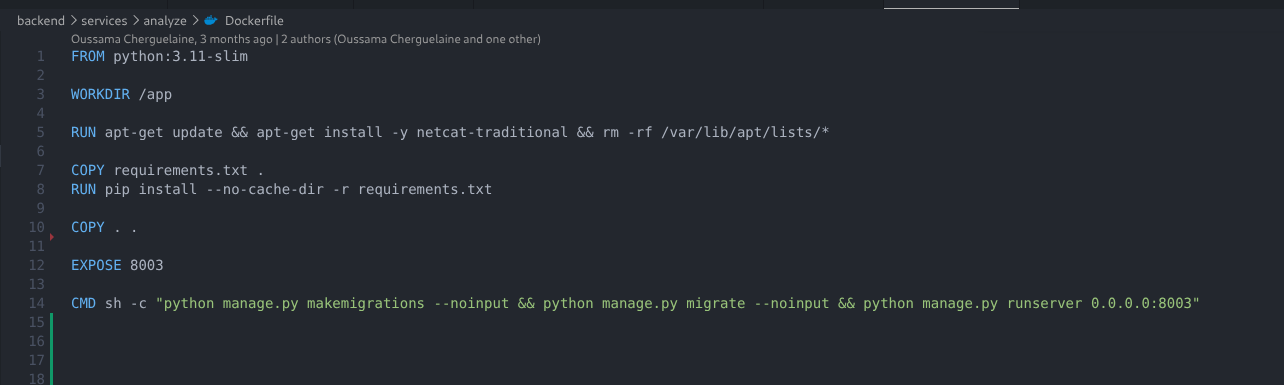
\includegraphics[width=0.95\textwidth]{captures/dockerfile_analyze.png}
    \caption{Structure du \texttt{Dockerfile} du service d'analyse de RevMine}
    \label{fig:dockerfile}
\end{figure}

% ============================================================
\section{Test}
% ============================================================

\subsection{Stratégie de test}

La stratégie de test adoptée pour RevMine s'articule autour de quatre niveaux complémentaires~:

\begin{itemize}
    \item \textbf{Tests unitaires}~: vérification isolée des fonctions, classes et composants
          individuels au sein de chaque service backend et du frontend~;
    \item \textbf{Tests d'intégration}~: validation des interactions entre les couches d'un même
          service~;
    \item \textbf{Tests fonctionnels (\textit{end-to-end})}~: simulation de scénarios utilisateur
          complets dans un environnement proche de la production, à l'aide de Cypress~;
    \item \textbf{Tests de non-régression}~: exécutés automatiquement à chaque commit via le
          pipeline GitLab CI.
\end{itemize}

Les outils de test mobilisés pour chacune des couches de la plateforme sont récapitulés dans le
Tableau~\ref{tab:outils-tests}.

\begin{table}[H]
\centering
\small
\caption{Outils de test utilisés dans RevMine}
\label{tab:outils-tests}
\begin{tabular}{|>{\raggedright\arraybackslash}p{3.5cm}
                |>{\raggedright\arraybackslash}p{3.8cm}
                |>{\raggedright\arraybackslash}p{5.5cm}|}
\hline
\textbf{Couche} & \textbf{Outil} & \textbf{Périmètre couvert} \\
\hline
Backend Python & pytest + pytest-django & Tests unitaires et d'intégration \\
\hline
Frontend React & Jest + React Testing Library & Tests des services et composants JS \\
\hline
End-to-End & Cypress & Scénarios fonctionnels complets \\
\hline
Qualité statique & SonarQube 10.4 & Couverture, bugs, \textit{code smells} \\
\hline
CI/CD & GitLab CI & Automatisation des tests et build Docker \\
\hline
Couverture & Cobertura (\texttt{coverage.xml}) & Rapports de couverture par service \\
\hline
Service LLM & Benchmark (500~scénarios) & Parsing langage naturel vers JSON conforme \\
\hline
\end{tabular}
\end{table}

\subsection{Tests unitaires}

Les tests unitaires constituent le premier niveau de validation. Dans RevMine, chaque service
backend dispose de son propre dossier de tests, organisé en fichiers thématiques et exécuté via
le framework \textbf{pytest}.

\subsubsection*{Service de configuration}

Le service de configuration dispose d'une suite de tests complète répartie sur sept fichiers,
organisés selon les couches de l'architecture propre (\textit{clean architecture}) adoptée,
comme présenté dans le Tableau~\ref{tab:tests-config}.

\begin{table}[H]
\centering
\small
\caption{Fichiers de tests du service de configuration}
\label{tab:tests-config}
\begin{tabular}{|>{\raggedright\arraybackslash}p{6cm}
                |>{\raggedright\arraybackslash}p{7cm}|}
\hline
\textbf{Fichier de test} & \textbf{Périmètre couvert} \\
\hline
\texttt{test\_api\_views.py} & Endpoints REST (CRUD workspaces et dépôts, test de connexion) \\
\hline
\texttt{test\_encryption.py} & Chiffrement et déchiffrement des tokens AES via Fernet \\
\hline
\texttt{test\_kafka\_handlers.py} & Publication et consommation sur les topics \texttt{config.tokens.*} \\
\hline
\texttt{test\_repository\_service.py} & Récupération et import des dépôts depuis GitHub et GitLab \\
\hline
\texttt{test\_workspace\_rules.py} & Règles métier (unicité du nom, validation de plateforme, URL) \\
\hline
\texttt{test\_workspace\_service.py} & Cycle de vie du workspace (création, test, mise à jour) \\
\hline
\texttt{test\_workspaces.py} & Tests d'intégration des couches combinées (suite héritée) \\
\hline
\end{tabular}
\end{table}

Cette suite totalise \textbf{88~tests}, dont 30~tests hérités et 58~nouveaux tests couvrant
l'architecture refactorisée.

\subsubsection*{Service de collecte}

Le service de collecte est structuré autour de cinq fichiers de tests thématiques, complétés
d'un fichier de fixtures partagées, comme détaillé dans le Tableau~\ref{tab:tests-collection}.

\begin{table}[H]
\centering
\small
\caption{Fichiers de tests du service de collecte}
\label{tab:tests-collection}
\begin{tabular}{|>{\raggedright\arraybackslash}p{4.5cm}
                |>{\raggedright\arraybackslash}p{8.5cm}|}
\hline
\textbf{Fichier de test} & \textbf{Périmètre couvert} \\
\hline
\texttt{test\_api.py} & Endpoints REST du workflow de collecte \\
\hline
\texttt{test\_domain.py} & Modèles de données et règles métier (\texttt{Collection}, \texttt{CleanedData}) \\
\hline
\texttt{test\_infrastructure.py} & Interactions avec MinIO (stockage et récupération de fichiers) \\
\hline
\texttt{test\_integration.py} & Flux d'exécution complets, de l'initialisation à la génération du CSV \\
\hline
\texttt{test\_services.py} & Logique des services métier (\texttt{CollectionService}, \texttt{DataCleaningService}) \\
\hline
\texttt{conftest.py} & Fixtures pytest partagées (base de données de test, clients simulés) \\
\hline
\end{tabular}
\end{table}

\subsubsection*{Service d'analyse}

Le service d'analyse dispose de la suite de tests la plus étendue, organisée en neuf fichiers
couvrant chaque couche de l'architecture, comme présenté dans le Tableau~\ref{tab:tests-analyze}.

\begin{table}[H]
\centering
\small
\caption{Fichiers de tests du service d'analyse}
\label{tab:tests-analyze}
\begin{tabular}{|>{\raggedright\arraybackslash}p{6cm}
                |>{\raggedright\arraybackslash}p{7cm}|}
\hline
\textbf{Fichier de test} & \textbf{Périmètre couvert} \\
\hline
\texttt{test\_metrics\_engine.py} & Calcul des 60+ métriques analytiques via le moteur \texttt{MetricsEngine} \\
\hline
\texttt{test\_dataset\_service.py} & Cycle de vie des datasets (création, chargement, suppression) \\
\hline
\texttt{test\_dataset\_loader.py} & Lecture CSV et détection des colonnes supplémentaires \\
\hline
\texttt{test\_analysis\_service.py} & Orchestration de l'analyse \\
\hline
\texttt{test\_analysis\_service\_new.py} & Tests complémentaires de la version refactorisée \\
\hline
\texttt{test\_celery\_tasks.py} & Tâches asynchrones Celery (déclenchement, exécution, erreurs) \\
\hline
\texttt{test\_api\_views.py} & Vues API (upload de dataset, génération de graphique, historique) \\
\hline
\texttt{test\_api.py} & Tests complémentaires des endpoints REST \\
\hline
\texttt{test\_shim\_compatibility.py} & Compatibilité des modules shims après refactorisation \\
\hline
\end{tabular}
\end{table}

\subsubsection*{Frontend}

La couche frontend est testée à l'aide de \textbf{Jest} et de \textbf{React Testing Library}.
Le fichier \texttt{src/services/api.test.js} valide le comportement de l'instance Axios
configurée~: injection automatique du token JWT dans l'en-tête \texttt{Authorization} et
rafraîchissement silencieux du token en cas d'expiration.

\subsection{Tests d'intégration}

Des bases de tests d'intégration ont été posées au sein de plusieurs services. Dans le service
de collecte, le fichier \texttt{test\_integration.py} valide le flux complet allant de
l'initialisation d'un plan de collecte à la génération du fichier CSV structuré. Dans le service
de configuration, le fichier \texttt{test\_kafka\_handlers.py} valide l'émission et la réception
de messages Kafka sur les topics \texttt{config.tokens.request} et
\texttt{config.tokens.response}.

\subsection{Tests fonctionnels (End-to-End)}

Les tests de bout en bout sont réalisés à l'aide de \textbf{Cypress}. Trois fichiers de tests
couvrent les scénarios les plus critiques de l'application, comme présenté dans le
Tableau~\ref{tab:tests-cypress}.

\begin{table}[H]
\centering
\small
\caption{Scénarios de tests fonctionnels end-to-end avec Cypress}
\label{tab:tests-cypress}
\begin{tabular}{|>{\raggedright\arraybackslash}p{4cm}
                |>{\raggedright\arraybackslash}p{9cm}|}
\hline
\textbf{Fichier Cypress} & \textbf{Scénarios couverts} \\
\hline
\texttt{auth.cy.js} & Inscription, connexion, déconnexion, refus d'accès aux routes protégées \\
\hline
\texttt{workspaces.cy.js} & Création de workspace, test de connexion, import de dépôts, suppression \\
\hline
\texttt{user-journey.cy.js} & Parcours complet~: authentification, workspace, collecte, résultats \\
\hline
\end{tabular}
\end{table}

\subsection{Qualité du code et analyse statique}

L'analyse statique est réalisée avec \textbf{SonarQube Community 10.4}. La configuration est
centralisée dans \texttt{sonar-project.properties} et couvre le répertoire \texttt{backend/}.
Le \textbf{Quality Gate} bloquant interrompt le pipeline CI/CD si les seuils ne sont pas
atteints, garantissant qu'aucun code ne franchit la barrière de l'intégration continue sans
satisfaire les critères requis. Le tableau de bord SonarQube est illustré à la
Figure~\ref{fig:sonar-dashboard}.

\begin{figure}[H]
    \centering
    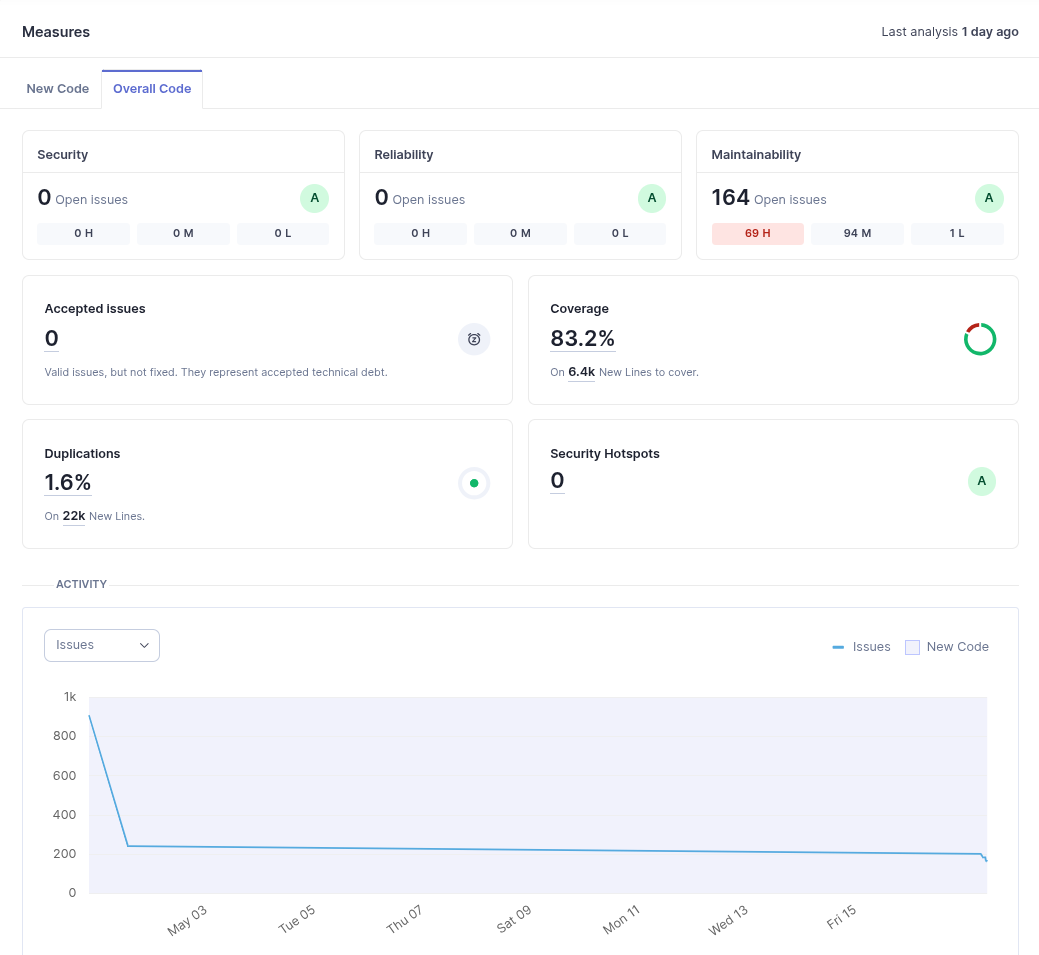
\includegraphics[width=0.95\textwidth]{captures/sonarqube_dashboard.png}
    \caption{Tableau de bord SonarQube -- métriques de qualité de RevMine}
    \label{fig:sonar-dashboard}
\end{figure}

% ============================================================
\section{Déploiement}
\label{sec:deploiement}
% ============================================================

Le déploiement de RevMine s'appuie sur deux piliers complémentaires~: l'orchestration des
conteneurs via \textbf{Docker Compose}, qui assure le démarrage coordonné de l'ensemble de la
stack en environnement local, et le pipeline CI/CD GitLab, qui automatise la validation et la
construction des livrables à chaque évolution du code.

\subsection{Orchestration avec Docker Compose}

Le fichier \texttt{docker-compose.yaml} est le point central de l'orchestration locale. Il
déclare l'ensemble des services, leurs dépendances de démarrage (\texttt{depends\_on}), les
variables d'environnement, les volumes persistants et le réseau Docker commun, garantissant que
les services d'infrastructure (bases de données, Kafka, MinIO) sont opérationnels avant le
démarrage des services applicatifs. Le Tableau~\ref{tab:docker-services} récapitule les services
orchestrés et leur rôle.

\begin{table}[H]
\centering
\small
\caption{Services orchestrés par Docker Compose dans RevMine}
\label{tab:docker-services}
\begin{tabular}{|>{\raggedright\arraybackslash}p{4cm}
                |>{\raggedright\arraybackslash}p{4cm}
                |>{\raggedright\arraybackslash}p{5cm}|}
\hline
\textbf{Service} & \textbf{Image / Technologie} & \textbf{Rôle} \\
\hline
\texttt{api-gateway} & Python 3.11 / Django & Point d'entrée unique, authentification JWT \\
\hline
\texttt{config-service} & Python 3.11 / Django & Gestion des workspaces et dépôts \\
\hline
\texttt{collection-service} & Python 3.11 / Django & Collecte et nettoyage des données \\
\hline
\texttt{analyze-service} & Python 3.11 / Django & Génération des analyses et graphiques \\
\hline
\texttt{llm-service} & Python 3.11 / FastAPI & Interface vers les modèles de langage \\
\hline
\texttt{notification-service} & Go 1.21 / Fiber & Notifications temps réel via WebSocket \\
\hline
\texttt{frontend} & Node.js / React & Interface utilisateur SPA \\
\hline
\texttt{db-gateway}, \texttt{db-config}, \texttt{db-collection}, \texttt{db-analyze} & PostgreSQL 15 & Bases de données isolées par service \\
\hline
\texttt{kafka} & Confluent Platform 7.5.0 & Bus de messages asynchrone (mode KRaft) \\
\hline
\texttt{minio} & MinIO & Stockage objet compatible S3 \\
\hline
\texttt{redis} & Redis 7 & Cache et broker Celery \\
\hline
\texttt{loki}, \texttt{promtail}, \texttt{grafana} & Grafana Stack & Collecte et visualisation des journaux \\
\hline
\end{tabular}
\end{table}

L'ensemble des services est regroupé dans un réseau Docker commun (\texttt{revmine-network}),
permettant aux conteneurs de communiquer entre eux par leur nom de service. Des volumes
persistants nommés sont définis pour les bases de données PostgreSQL, MinIO et Grafana,
garantissant la conservation des données entre les redémarrages.

Chaque service reçoit sa configuration via des variables d'environnement déclarées dans le
fichier \texttt{.env}, chargé automatiquement par Docker Compose. Cette approche garantit que
les secrets (clés API, mots de passe, clé Fernet) ne sont jamais inclus dans le code source
ni dans les images Docker.

Le démarrage complet de la stack s'effectue par la commande~:

\begin{verbatim}
docker compose up --build
\end{verbatim}

La Figure~\ref{fig:docker-compose-up} illustre le démarrage de la stack complète, montrant la
mise en ligne séquentielle et ordonnée de l'ensemble des conteneurs.

\begin{figure}[H]
    \centering
    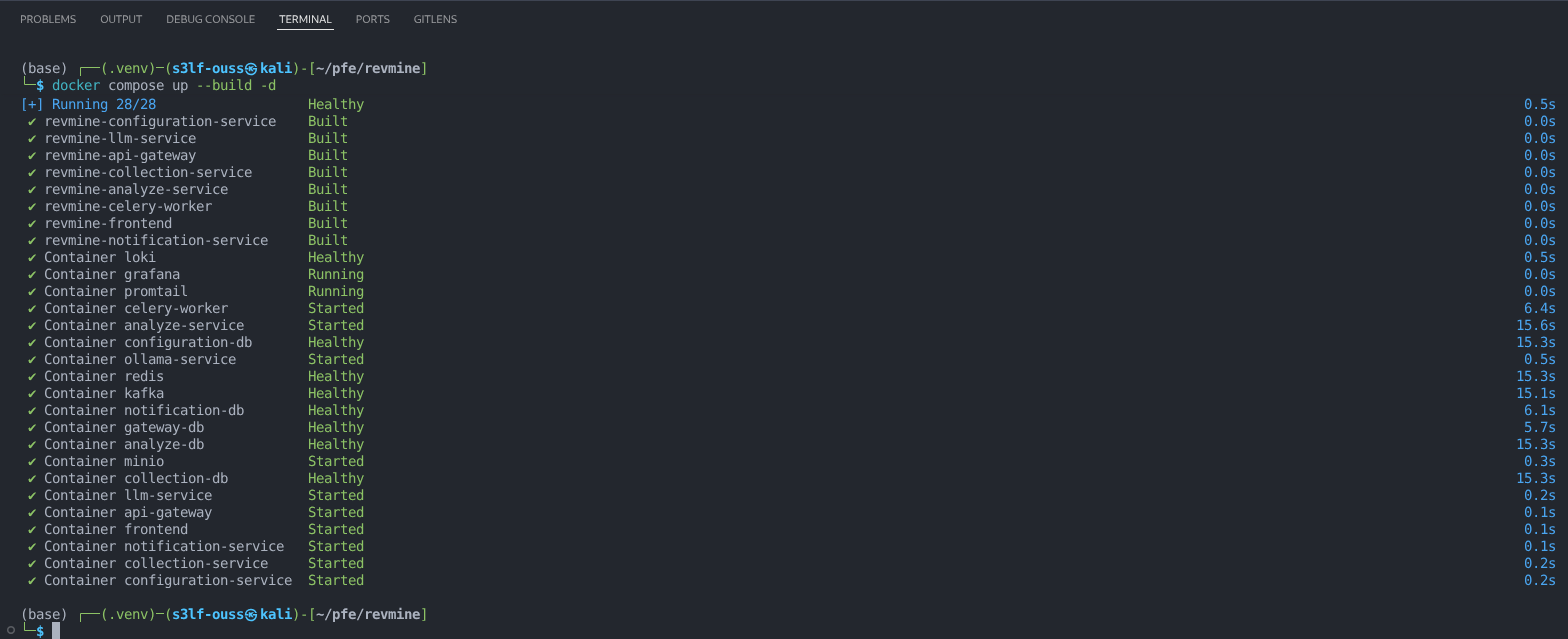
\includegraphics[width=0.95\textwidth]{captures/docker_compose_up.png}
    \caption{Démarrage de la stack RevMine avec Docker Compose}
    \label{fig:docker-compose-up}
\end{figure}

Les points d'accès exposés par la stack déployée sont les suivants~:

\begin{itemize}
    \item \textbf{Frontend React}~: \texttt{http://localhost:3000}~;
    \item \textbf{API Gateway}~: \texttt{http://localhost:8000}~;
    \item \textbf{MinIO Console}~: \texttt{http://localhost:9001}~;
    \item \textbf{Grafana}~: \texttt{http://localhost:3100}~;
    \item \textbf{SonarQube}~: \texttt{http://localhost:9000}.
\end{itemize}

La Figure~\ref{fig:docker-ps} illustre l'état de la stack RevMine à l'aide de la commande \texttt{docker ps},
montrant l'ensemble des conteneurs en cours d'exécution ainsi que leur état respectif.
\begin{figure}[H]
\centering
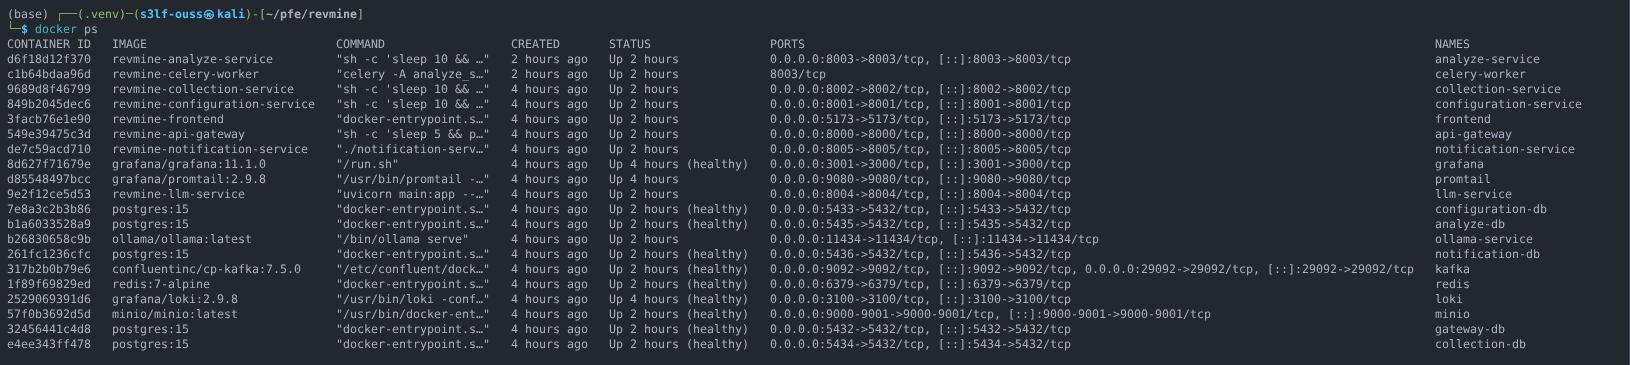
\includegraphics[width=0.95\textwidth]{captures/docker_ps_stack.png}
\caption{Stack RevMine déployée -- état des conteneurs via la commande \texttt{docker ps}}
\label{fig:docker-ps}
\end{figure}

\subsection{Pipeline CI/CD}
\label{subsec:cicd}

Le pipeline d'intégration et de livraison continues (CI/CD\footnote{CI/CD~: \textit{Continuous
Integration / Continuous Delivery}. L'intégration continue consiste à automatiser la vérification
du code à chaque modification~; la livraison continue étend cette automatisation jusqu'à la
construction des livrables déployables.}) de RevMine est défini dans le fichier
\texttt{.gitlab-ci.yml}. Il s'organise en trois étapes successives~: \textbf{test},
\textbf{qualité} et \textbf{build}, dont les responsabilités sont détaillées dans le
Tableau~\ref{tab:pipeline-ci}.

\begin{table}[H]
\centering
\small
\caption{Étapes du pipeline GitLab CI de RevMine}
\label{tab:pipeline-ci}
\begin{tabular}{|>{\raggedright\arraybackslash}p{2cm}
                |>{\raggedright\arraybackslash}p{4.5cm}
                |>{\raggedright\arraybackslash}p{6.5cm}|}
\hline
\textbf{Étape} & \textbf{Job(s)} & \textbf{Description} \\
\hline
\texttt{test} & \texttt{test:all} & Exécution des tests unitaires de tous les services backend \\
\hline
\texttt{quality} & \texttt{sonar:scan} & Analyse SonarQube et validation du Quality Gate \\
\hline
\texttt{build} & \makecell[l]{\texttt{build:api-gateway} \\ \texttt{build:analyze} \\ \texttt{build:configuration} \\ \texttt{build:collection}} & Construction des images Docker (branches \texttt{main}/\texttt{master} uniquement) \\
\hline
\end{tabular}
\end{table}

\paragraph{Étape de test.} Le job \texttt{test:all} s'exécute sur une image
\texttt{python:3.11-slim} avec un service PostgreSQL~15 comme base de données de test. Il
provisionne les quatre bases de données nécessaires (\texttt{gateway\_db}, \texttt{analyze\_db},
\texttt{configuration\_db}, \texttt{collection\_db}), puis lance séquentiellement les tests pour
chaque service backend. Les rapports JUnit (\texttt{junit-report.xml}) et Cobertura
(\texttt{coverage.xml}) sont conservés comme artefacts dans GitLab pendant une semaine.

\paragraph{Étape d'analyse qualité.} L'étape \texttt{quality} exécute le scanner SonarQube en
s'appuyant sur les rapports de couverture générés lors de l'étape précédente. Le Quality Gate
bloquant interrompt le pipeline si les seuils ne sont pas atteints.

\paragraph{Étape de build Docker.} Déclenchée uniquement sur les branches \texttt{main} ou
\texttt{master}, elle construit les images Docker pour les quatre services backend principaux,
chacun disposant de son propre \texttt{Dockerfile} basé sur \texttt{python:3.11-slim}.

Les Figures~\ref{fig:pipeline-passed} et~\ref{fig:pipeline-failed} illustrent respectivement
une exécution réussie et un exemple d'échec détecté par le pipeline.

\begin{figure}[H]
    \centering
    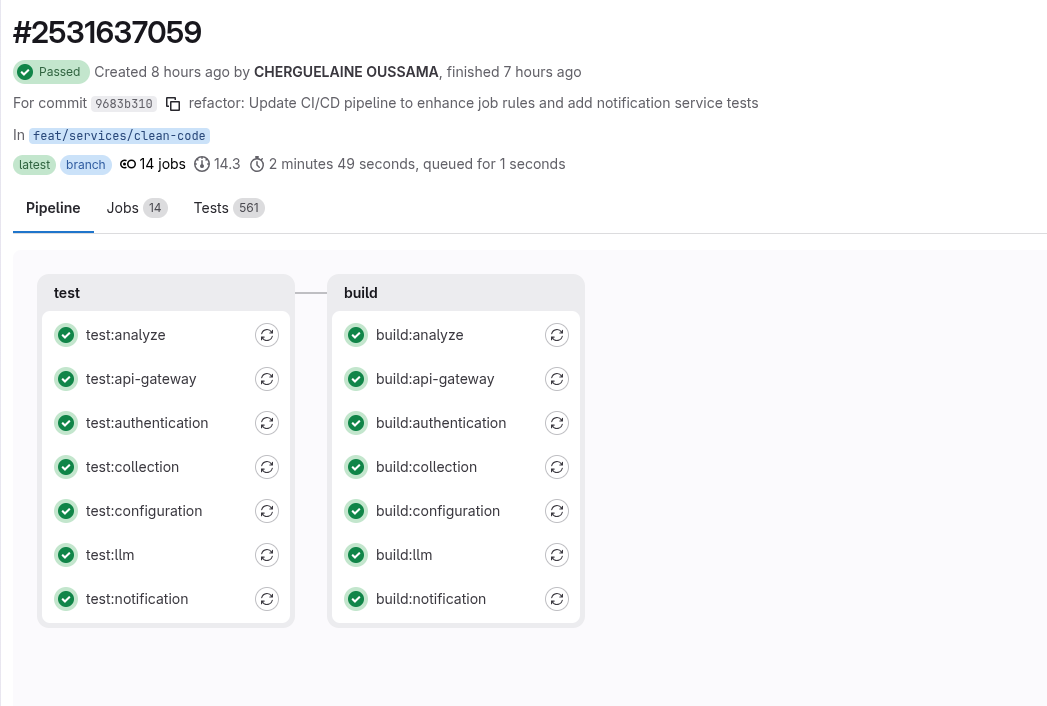
\includegraphics[width=0.95\textwidth]{captures/gitlab_pipeline_passed.png}
    \caption{Pipeline GitLab CI -- exécution réussie (toutes les étapes validées)}
    \label{fig:pipeline-passed}
\end{figure}

\begin{figure}[H]
    \centering
    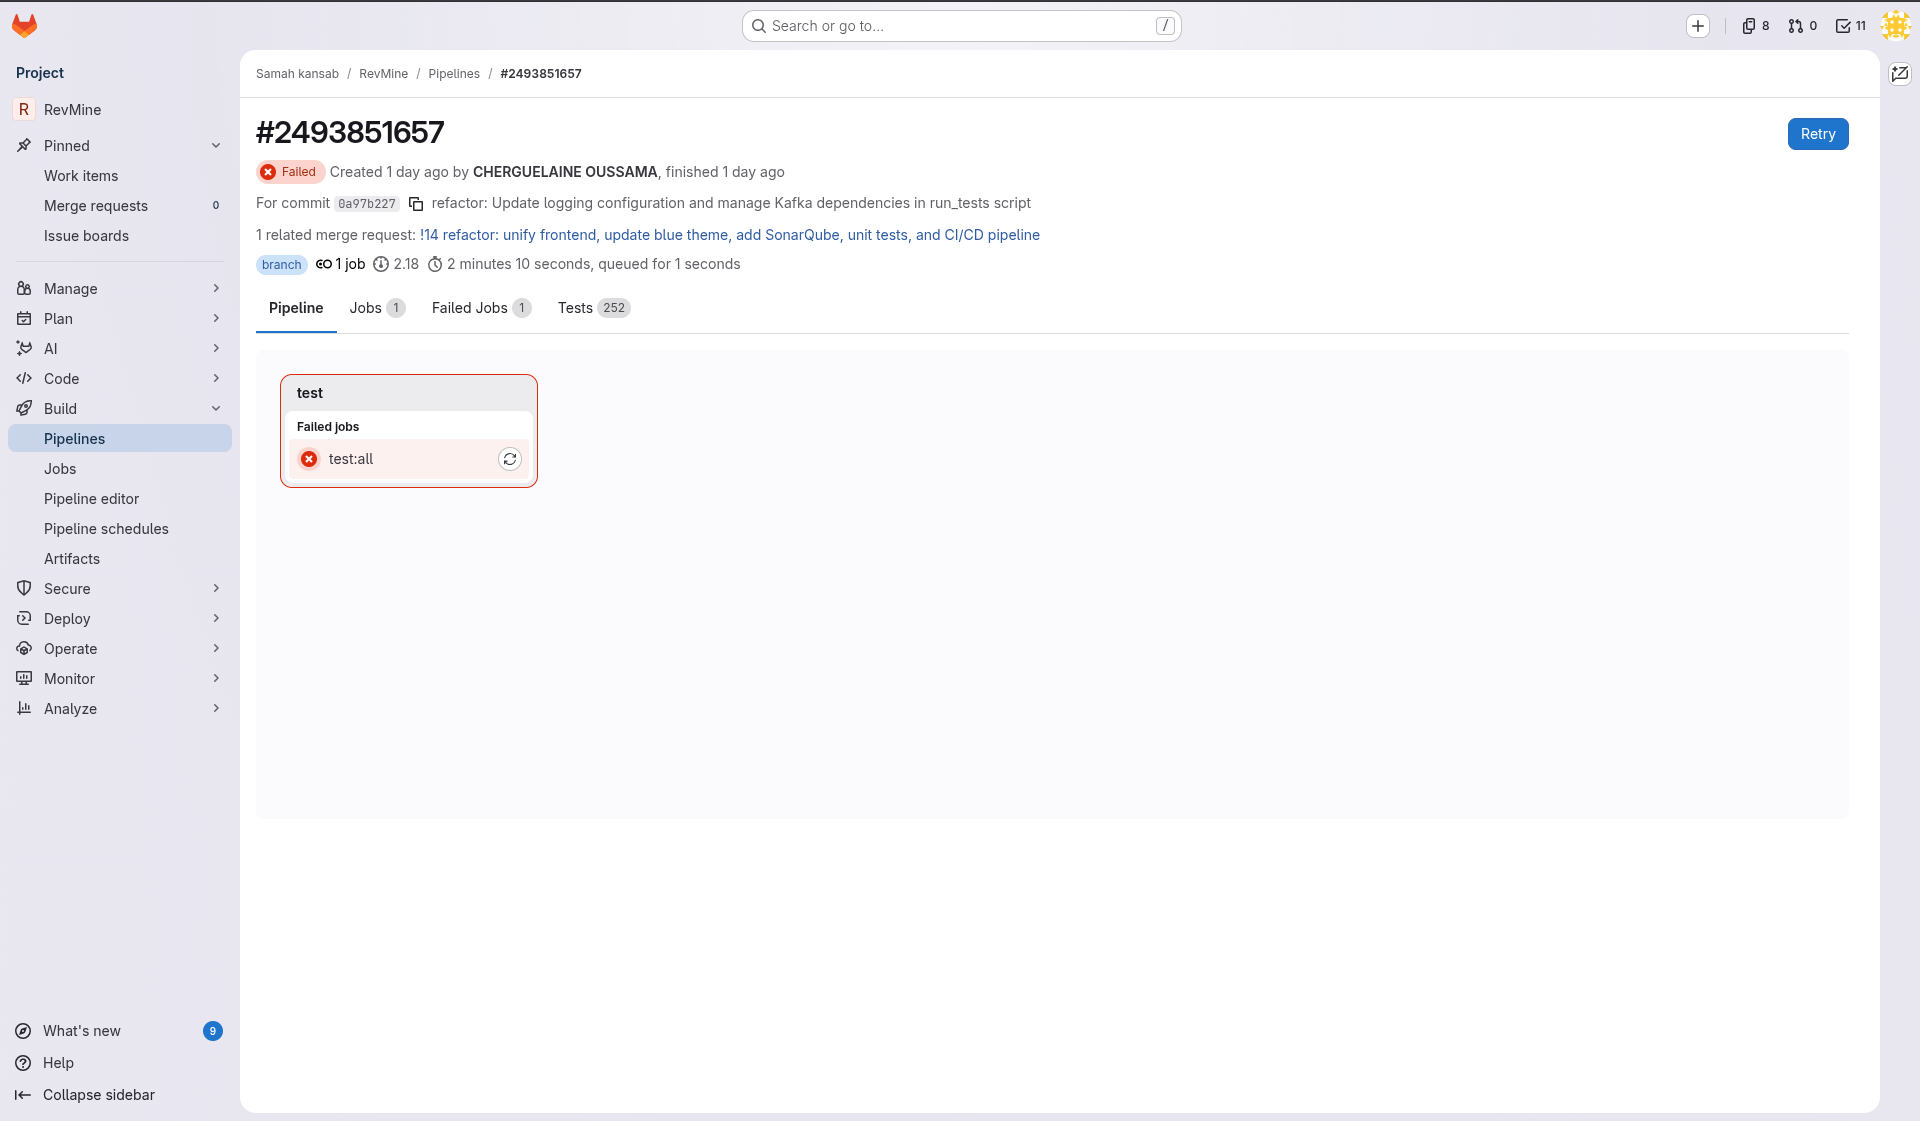
\includegraphics[width=0.95\textwidth]{captures/gitlab_pipeline_failed.png}
    \caption{Pipeline GitLab CI -- exemple d'échec détecté par le pipeline}
    \label{fig:pipeline-failed}
\end{figure}

% ============================================================
% Section : Surveillance et Observabilité
% ============================================================
\section{Surveillance}
\label{sec:surveillance}

\subsection{Architecture d'observabilité}

La surveillance de la plateforme RevMine repose sur la pile \textbf{Loki + Promtail + Grafana}, présentée à la section~\ref{subsec:grafana-tech}. Cette architecture centralise la collecte, le stockage et la visualisation des journaux de tous les microservices dans une interface unifiée.

Chaque service de RevMine est configuré pour produire ses journaux en \textbf{JSON structuré}, incluant systématiquement le niveau de sévérité (\texttt{DEBUG}, \texttt{INFO}, \texttt{WARNING}, \texttt{ERROR}), l'horodatage, le nom du service et le message. Cette structuration permet à Grafana d'appliquer des filtres précis via le langage de requête \textbf{LogQL} et de construire des tableaux de bord d'observabilité détaillés.

\subsection{Tableaux de bord Grafana}

Plusieurs tableaux de bord ont été configurés pour couvrir les dimensions techniques, applicatives et financières de la plateforme.

\subsubsection{Vue d'ensemble et état de santé}
Le tableau de bord principal offre une vue consolidée de l'état de santé de l'ensemble de la plateforme. Il agrège les journaux et permet d'identifier en un coup d'œil les anomalies survenues sur une période donnée.

\begin{figure}[H]
    \centering
    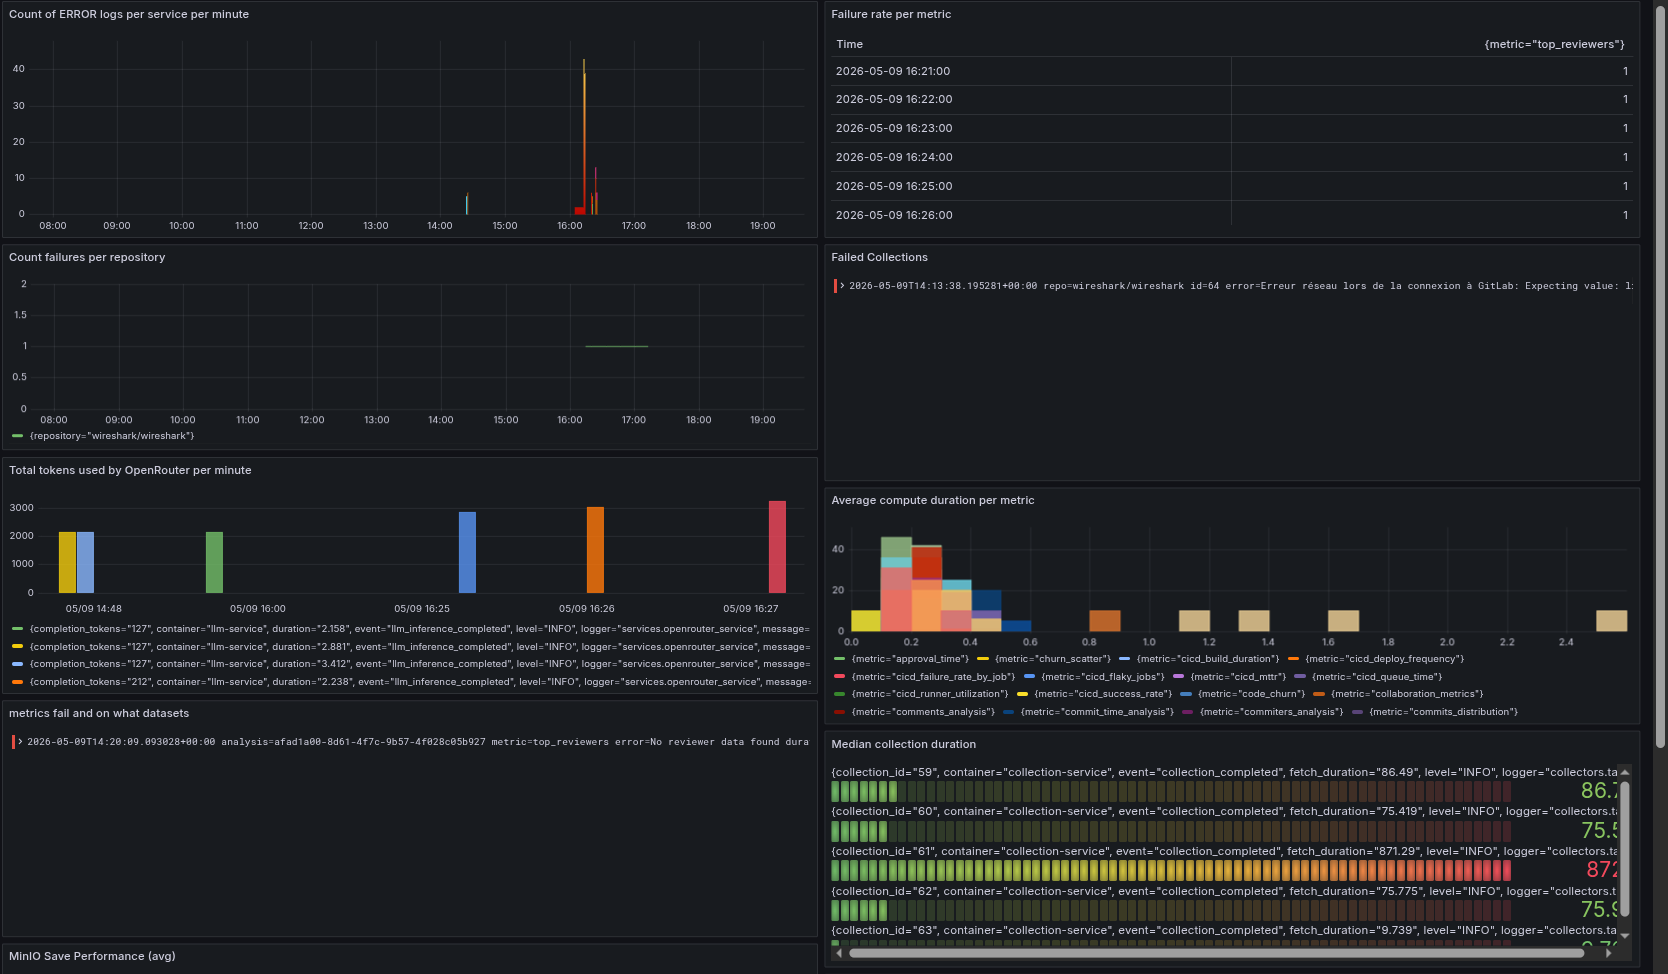
\includegraphics[width=0.95\textwidth]{captures/grafana_overview_dashboard.png}
    \caption{Tableau de bord Grafana -- Vue d'ensemble de la plateforme RevMine}
    \label{fig:grafana-overview}
\end{figure}

\subsubsection{Surveillance par service et flux de logs}
Des panels dédiés permettent de filtrer les journaux par microservice. Pour chaque service, les métriques suivantes sont visualisées :
\begin{itemize}
    \item le \textbf{volume de journaux} par unité de temps ;
    \item la \textbf{distribution des niveaux de sévérité} (ratio INFO / ERROR) ;
    \item le \textbf{flux en temps réel} pour le diagnostic à chaud.
\end{itemize}

\begin{figure}[H]
    \centering
    
\includegraphics[width=0.95\textwidth]{captures/grafana_service_logs.png}
    \caption{Panel Grafana -- Focus sur le service de collecte}
    \label{fig:grafana-service}
\end{figure}

\subsubsection{Indicateurs de performance et de consommation (Performance \& Costs)}
Pour affiner le pilotage de la plateforme, un tableau de bord spécifique suit les indicateurs de performance algorithmique et l'utilisation des ressources :

\begin{itemize}
    \item \textbf{Temps moyen de calcul par métrique} : Mesure la latence d'exécution de chaque algorithme dans le service d'analyse pour identifier les goulots d'étranglement.
    \item \textbf{Temps moyen de collection par dépôt} : Évalue l'efficacité du service de collecte en fonction de la taille des dépôts traités.
    \item \textbf{Consommation de tokens LLM} : Suit l'utilisation des jetons via l'API OpenRouter, permettant de monitorer les coûts liés à l'intelligence artificielle.
\end{itemize}

\begin{figure}[H]
    \centering
    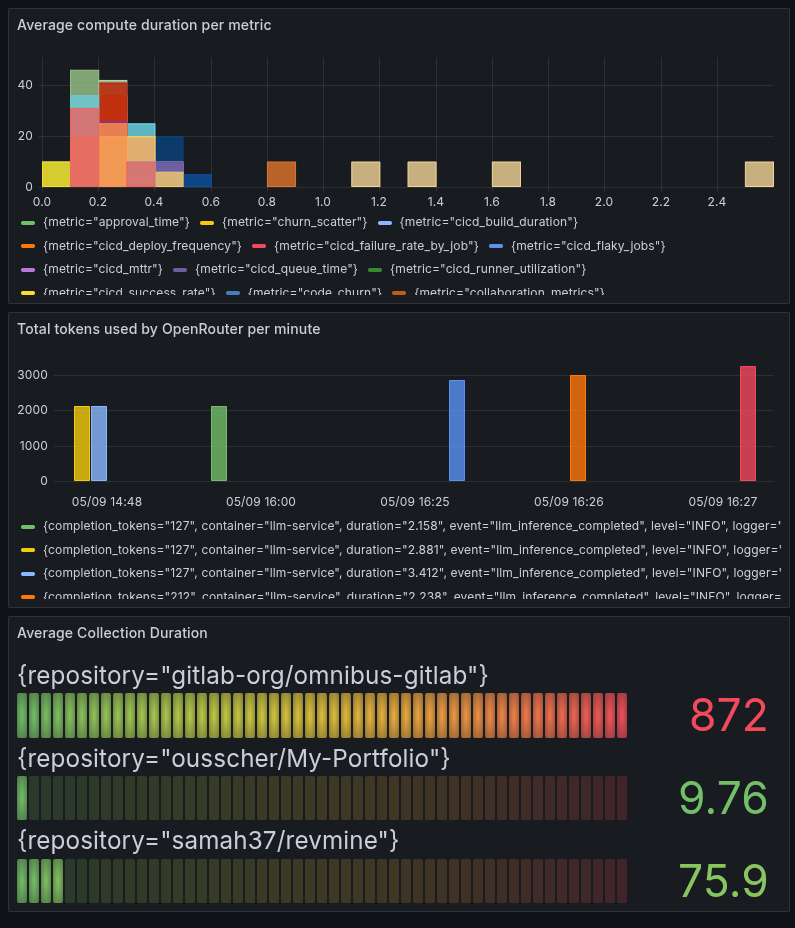
\includegraphics[width=0.95\textwidth]{captures/grafana_performance_costs.png}
    \caption{Panel Grafana -- Analyse des performances et consommation de tokens LLM}
    \label{fig:grafana-perf-costs}
\end{figure}

\subsubsection{Gestion des erreurs applicatives}
Un panel dédié agrège les entrées \texttt{ERROR} et \texttt{WARNING}. Il est crucial pour identifier les défaillances lors des communications Kafka ou des échecs d'analyse sémantique.

\begin{figure}[H]
    \centering
    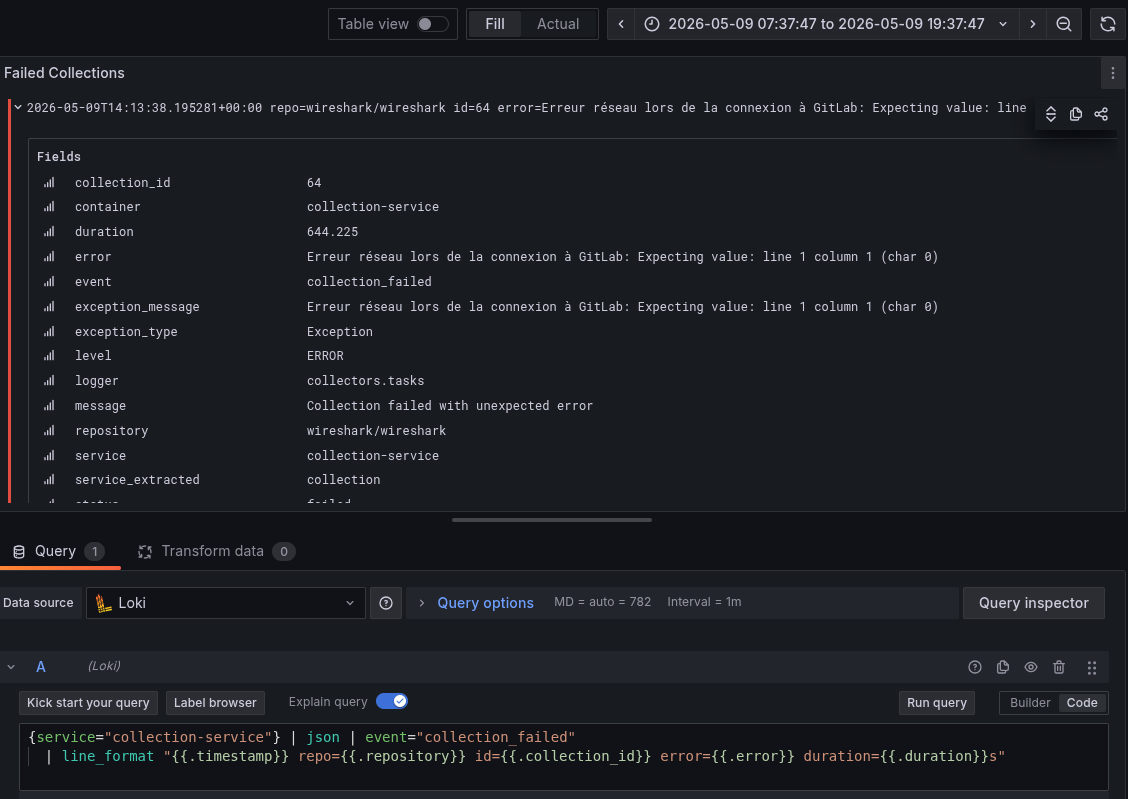
\includegraphics[width=0.95\textwidth]{captures/grafana_errors_panel.png}
    \caption{Panel Grafana -- Agrégation et détection des erreurs critiques}
    \label{fig:grafana-errors}
\end{figure}

\subsection{Interprétation et utilité opérationnelle}

L'observabilité mise en place dans RevMine répond à quatre besoins majeurs :

\begin{itemize}
    \item \textbf{Détection proactive} : Identification immédiate d'un crash service via les pics d'erreurs.
    \item \textbf{Optimisation des performances} : Le suivi des temps de calcul permet d'isoler les métriques les plus lourdes et d'envisager des optimisations ou une mise à l'échelle (scaling).
    \item \textbf{Maîtrise des coûts} : Le monitoring des tokens OpenRouter offre une visibilité financière indispensable pour l'utilisation des modèles de langage en production.
    \item \textbf{Traçabilité} : L'utilisation d'IDs structurés permet de suivre une requête utilisateur de la collecte jusqu'à l'affichage final des résultats.
\end{itemize}
% ============================================================
\section{Conclusion}
% ============================================================

La phase de réalisation de RevMine a permis de concrétiser l'architecture microservices définie
lors de la conception en une solution fonctionnelle, modulaire et évolutive. Développé en binôme,
le projet a bénéficié d'une organisation rigoureuse~: convention de branches justifiée, revues de
code systématiques, sprints hebdomadaires et réunions mensuelles avec l'encadrant de l'ETS.

Le choix de technologies complémentaires et adaptées à chaque périmètre -- Python/Django pour les
services métier, FastAPI pour le service LLM, Go pour les notifications temps réel, React pour le
frontend, et la pile Grafana~+~Loki~+~Promtail pour l'observabilité -- a permis de répondre aux
exigences de performance, de maintenabilité et de flexibilité.

La culture DevOps adoptée, structurée autour du cycle Plan~→~Code~→~Build~→~Test~→~Deploy~→~Operate~→~Feedback~→~Monitor, se matérialise concrètement par une conteneurisation systématique via Docker et un pipeline GitLab CI avec Quality Gate SonarQube bloquant, qui garantissent qu'aucun code dégradé ne passe en intégration et que les images produites sont toujours reproductibles.

Enfin, la stratégie de test multi-niveaux -- des tests unitaires aux scénarios end-to-end en
passant par l'évaluation empirique du service LLM sur 500~scénarios -- associée à la surveillance
continue via Grafana, pose les fondements d'une plateforme fiable et maintenable, capable
d'intégrer de nouvelles fonctionnalités sans compromettre la qualité de l'existant.